\documentclass[preprint,12pt]{elsarticle}
\usepackage[utf8]{inputenc}
\usepackage[T1]{fontenc}
\usepackage{lmodern}
\usepackage{amsmath,amssymb,amsthm}
\usepackage{xcolor,graphicx,enumerate}
\usepackage{algorithm,algpseudocode}
\usepackage{enumitem}
\usepackage{booktabs,tabularx,array,ragged2e}
\usepackage{tikz}
\usepackage{caption,subcaption}
\usepackage{float,longtable,pdflscape}
\usepackage{siunitx}
\usepackage{xurl}
\usepackage{hyperref}
\graphicspath{{./}{./figures/}}
\sisetup{per-mode=symbol}
\newcolumntype{L}[1]{>{\RaggedRight\arraybackslash}p{#1}}
\newcolumntype{Y}{>{\RaggedRight\arraybackslash}X}
\usetikzlibrary{shapes,arrows.meta,positioning}
\newcommand{\SafeIncludeGraphics}[2][]{\IfFileExists{#2}{\includegraphics[#1]{#2}}{\PackageError{ACLD}{Missing research figure #2}{Supply the required figure file}}}
\newcommand{\SafeInput}[1]{\IfFileExists{#1}{\input{#1}}{\PackageError{ACLD}{Missing research table #1}{Supply the required research table}}}
\newif\ifcolor\colortrue
\newcommand{\plExp}{\xi}
\newcommand{\degIn}[1]{\mathrm{deg}_{\mathrm{in}}(#1,t)}
\newcommand{\Nbr}[1]{\mathcal N_{#1}(t)}
\theoremstyle{definition}\newtheorem{definition}{Definition}
\theoremstyle{plain}\newtheorem{theorem}{Theorem}
\theoremstyle{plain}\newtheorem{lemma}{Lemma}
\theoremstyle{plain}\newtheorem{corollary}{Corollary}
\theoremstyle{plain}\newtheorem{assumption}{Assumption}
\theoremstyle{remark}\newtheorem{remark}[theorem]{Remark}
\newcommand{\artifactRepo}{\url{https://github.com/ercanerkalkan/UavSwarmCriticalLinkDetection}}
\newcommand{\JNR}{\mathrm{JNR}}
\newcommand{\NF}{\mathrm{NF}}
\newcommand{\NB}{N_B}
\hypersetup{pdftitle={ACLD: Risk-Gated Partition Early Warning from Forecast Bridges in UAV Swarm Networks},pdfauthor={Ercan Erkalkan},colorlinks=true,linkcolor=blue,citecolor=blue,urlcolor=blue}

\setcounter{topnumber}{4}
\setcounter{bottomnumber}{2}
\setcounter{totalnumber}{6}
\renewcommand{\topfraction}{.9}
\renewcommand{\bottomfraction}{.8}
\renewcommand{\textfraction}{.08}
\renewcommand{\floatpagefraction}{.78}
\begin{document}
\setlength{\emergencystretch}{3em}
\begin{frontmatter}
\title{ACLD: Risk-Gated Partition Early Warning from Forecast Bridges in UAV Swarm Networks}
\author[aff1]{Ercan Erkalkan\corref{cor1}}
\cortext[cor1]{Corresponding author}
\ead{ercan.erkalkan@marmara.edu.tr}
\affiliation[aff1]{organization={Department of Electronics and Automation, Vocational School of Technical Sciences, Marmara University},addressline={Mehmet Gen\c{c} Campus},city={Istanbul},postcode={34865},country={Türkiye}}
\begin{abstract}
Forecasting network fragmentation in mobile UAV swarms requires separating next-step bridge localization from binary partition-warning decisions. Adaptive Critical Link Detection (ACLD) was evaluated as a logically centralized forecast-graph analyzer with a risk-gated warning policy. Seven synthetic simulation campaigns were analyzed with retained provenance records. Across 720 matched A2 scenario--seed units, ACLD and predictive Tarjan selected identical bridge sets (edge F1 = 0.99605), whereas the respective pooled warning false-positive rates were 0.03865 and 0.20434. In 40 additional S2 scenario--seed units (10 distinct seed identifiers, 159,960 transitions), the full-label ACLD/Tarjan comparison yielded 122/718 false positives and 1/0 false negatives. Because 98.09\% of transitions were already partition-positive, a retrospective onset analysis restricted the population to currently connected states: among 46 new disconnections, ACLD detected 45 with 117 false alerts, compared with 46 and 712 for predictive Tarjan; the respective false-positive rates were 3.84\% and 23.34\%. A components-only policy had fewer false alerts but missed more onsets, indicating a cost-dependent trade-off. Seed-cluster bootstrap intervals account for the 10 shared seed identifiers across scenario strata. Supporting controller experiments yielded connected-fraction gains of 0.187 and 0.046 percentage points; median desktop core execution was 58.015 ms at 150 UAVs and 3751.072 ms at 1000 UAVs, and intermediate-score calibration deviations remained. The evidence quantifies an early partition-warning policy under one-step synthetic network conditions, with optimized execution and deployment validation representing distinct assessment tasks.
\end{abstract}
\begin{keyword}
UAV swarm \sep flying ad hoc network \sep partition early warning \sep bridge localization \sep network reliability \sep false-positive rate
\end{keyword}
\end{frontmatter}
\section{Introduction}
Maintaining robust connectivity in Flying Ad Hoc Networks (FANETs) is a core requirement for mission-critical swarms deployed in search--rescue, surveillance, inspection, and emergency response scenarios~\cite{ranga2013network,rukaiya2024sdr}. FANET topologies evolve rapidly due to high mobility, tight control cycles, and volatile wireless conditions~\cite{yang2024pica}; consequently, a single link disruption may partition the swarm before conventional routing convergence. For FANET operation, \emph{proactive} link monitoring aims to anticipate imminent disconnections, rather than reacting after packet losses accumulate. An \emph{online} method makes a warning decision within each control cycle, without relying on offline recomputation or long-horizon future knowledge. Recent comparative studies further emphasize that FANETs extend MANET principles under stricter latency and congestion constraints in dense aerial settings~\cite{romero2025FANET,garciagil2024latency}.

A large body of work has addressed resilience using algebraic-connectivity metrics, adaptive routing, or learning-assisted policies~\cite{alenazi2023system,bai2024adaptive,bouziane2025routing,tho2025gpsrcb}. Classical graph vulnerability measures and adaptive wireless routing address related but different tasks; direct comparison with partition-warning rules requires a common prediction target~\cite{tarjan1972dfs,brandes2001betweenness,bai2024adaptive}. Snapshot-based approaches, in particular, do not directly predict future channel-viable edges, while FANET operation exhibits two recurring sources of mismatch: (i) the connectivity state at time $t$ may be invalid at $t+\Delta t_{\text{ctrl}}$ due to kinematic divergence; and (ii) fading and interference can invalidate purely geometric adjacency decisions~\cite{gashaw2025urban}. Classical graph primitives can indeed identify critical structures in a static snapshot, including bridges and articulation points via Tarjan-style DFS, edge-betweenness via Brandes, or global min-cut / $k$-edge-connectivity
methods such as Stoer--Wagner and Nagamochi--Ibaraki~\cite{tarjan1972dfs,brandes2001betweenness,stoer1997mincut,nagamochi1992edgeconn}. However, snapshot-only graph methods do not directly account for near-future topology evolution and channel uncertainty---two relevant factors in partition events for high-mobility aerial swarms.

Adaptive Critical Link Detection (ACLD) is examined as a logically centralized forecast-bridge localization and risk-gated partition-warning pipeline. At each decision step, a one-step kinematic forecast and a channel-viability criterion construct a predicted graph. Classical bridge extraction then identifies forecast-critical edges. The selected edge set is identical to the set produced by the matched predictive Tarjan baseline; the empirically distinguishable component is the binary partition-warning policy. Consequently, localization performance and false-positive warning rates are evaluated as separate tasks with separate denominators. The Python reference implementation is evaluated under a documented desktop timing protocol.

The empirically supported contributions are:
\begin{itemize}[leftmargin=*]
  \item \textbf{Explicit separation of localization and warning:} The predicted viable-graph bridge set is distinguished from the risk-gated binary partition decision, avoiding the inference that a lower warning false-positive rate reflects a novel edge-localization primitive.
  \item \textbf{Exact-label, denominator-aware evaluation:} Bridge-localization micro-F1 is computed from exact next-step bridge counts; warning metrics disclose event prevalence, negative support and aggregation conventions. An additional, explicitly retrospective S2 onset analysis restricts evaluation to currently connected states.
  \item \textbf{Paired robustness and controller analysis:} Matched scenario/seed comparisons cover mobility density, interference, a deterministic Rician-to-Nakagami viability approximation, ablations, and modest closed-loop control effects, with seed clustering and experimental provenance documented.
  \item \textbf{Runtime and reliability characterization:} A fully checkpointed 5,000-run core benchmark characterizes desktop scaling, while a separately fitted sigmoid score mapping is evaluated on disjoint seed cohorts and reliability deviations at sparsely supported score levels are reported.
  \item \textbf{Auditable artifact chain:} Validated episode/step records, source snapshots, uncertainty analyses, controlled data handling, and manuscript tables/figures are retained with explicit identification of P0.4/P0.5 and P0.6 campaign origins rather than reassignment of simulation provenance.
\end{itemize}

\paragraph{Research questions.}
Five research questions structure the evaluation:
\begin{description}[leftmargin=1.15cm,labelwidth=0.95cm,font=\normalfont\bfseries]
  \item[RQ1.] Accuracy of one-step partition-onset warnings conditioned on current network connectivity, relative to persistent-disconnection classification.
  \item[RQ2.] Attribution of observed differences to partition-warning decisions versus forecast-bridge localization.
  \item[RQ3.] Sensitivity of warning and localization metrics to swarm density, network size, fading assumptions and interference stress.
  \item[RQ4.] Observed controller-level effects of integrating ACLD alarms into a bounded mitigation policy relative to non-ACLD baselines.
  \item[RQ5.] Computational, calibration and communication-estimation limits of the evaluated implementation.
\end{description}

The manuscript is organized as follows. Section~\ref{sec:lit_comparative_summary}
reviews related work with emphasis on connectivity maintenance under dynamics and uncertainty.
Section~\ref{sec:system_architecture} makes the execution and adaptation architecture explicit.
Section~\ref{sec:methodology} details ACLD and the risk-cataloguing pipeline. Section~\ref{sec:simulation}
presents campaign results and retrospective onset evidence. Section~\ref{sec:Conclusion} concludes within the validated scope.

\section{Related Work and Positioning}\label{sec:lit_comparative_summary}

Work on flying ad hoc networks (FANETs) addresses several distinct goals: identifying structurally important nodes or edges, predicting topology transitions, maintaining connectivity through motion or radio control, and restoring connectivity after failures~\cite{yanmaz2022relay,yanmaz2023joint,luo2025isac}. Structural detection, proactive warning, connectivity maintenance and recovery have different outcome measures~\cite{guven2024multiobjective}. Classical bridge extraction and articulation-point identification are established graph primitives~\cite{tarjan1972dfs}; betweenness and cut formulations provide other structural references~\cite{brandes2001betweenness,stoer1997mincut,nagamochi1992edgeconn}. ACLD applies established bridge extraction to a one-step predicted channel-viable graph and evaluates a separate risk-gated warning rule.

\subsection{Connectivity preservation and topology repair}
Liu and Zhang~\cite{liu2022robust} developed a distributed node-importance and algebraic-connectivity approach for maintaining connectivity in mobile UAV swarms, with MATLAB simulations and a line-of-sight channel assumption. The distributed method addresses vulnerability to node failures and distributed control, whereas ACLD evaluates a logically centralized next-step warning decision over a predicted graph. Zear and Ranga~\cite{zear2022UAVs} proposed UAV-NetRest for detecting and reconnecting partitions in wireless sensor/actor networks. UAV-NetRest reports recovery time, relay UAV deployment, transmitted messages and traveled distance, rather than ACLD's binary warning endpoints. Li et al.~\cite{li2025fast} combined multi-agent deep deterministic policy gradients and artificial potential fields for distributed connectivity restoration following UAV failures; the PyTorch evaluation considers movement distance and recovery performance. The MADDPG--APF approach targets post-failure restoration rather than one-step pre-failure warning.

Related but non-equivalent work includes dynamic prediction-network identification of critical drones~\cite{teng2024communication}, localized critical-node detection using partial routing information~\cite{jin2017localized}, relay reconstruction~\cite{park2018droneNetXNR}, attack-resilient pairwise communication games~\cite{yang2019attack} and UAV-assisted software-defined WSN collection~\cite{Karegar2025Wireless}. The related methods motivate topology-aware analysis, although published outcomes cannot be compared numerically with ACLD warning false-positive rates without common tasks and data.

\subsection{Specific contribution relative to the nearest matched baseline}
The nearest matched experimental comparator is \emph{predictive Tarjan with the same forecast viable graph}. Both identify exactly the same bridges in the matched test. The testable difference lies in the binary warning policy. ACLD combines predicted component disconnection with a bridge--intercomponent-risk conjunction, whereas the matched Tarjan policy warns on any predicted bridge. The spectral and predicted-component criteria coincided in the recorded A2 and S2 scenario families, making the bridge--risk conjunction the identifiable warning-rule component. A components-only comparator and decision-cost analysis characterize the observed balance between false alerts and missed new partitions. The comparative contribution therefore concerns binary warning decisions over matched forecast bridges.

\begin{table}[htbp]
\centering\footnotesize
\caption{Related approaches to UAV and wireless-network connectivity. Different prediction and control objectives preclude direct numerical ranking across separate studies.}
\label{tab:related_comparison}
\begin{tabularx}{\linewidth}{@{}p{2.25cm}Y Y@{}}\toprule
Study & Main task and approach & Relation to ACLD\\\midrule
Liu and Zhang~\cite{liu2022robust} (2022) & Distributed node importance and algebraic-connectivity maintenance; MATLAB simulations & Maintains connectivity via distributed control; does not evaluate the matched ACLD warning rule\\
Zear and Ranga~\cite{zear2022UAVs} (2022) & UAV-assisted partition detection and \emph{post-failure} WSN connectivity restoration & Measures restoration, relay and communication costs instead of onset-warning FP/FN\\
Li et al.~\cite{li2025fast} (2025) & Distributed MADDPG--APF swarm connection restoration after UAV failure & Recovery-time/distance outcomes; not a pre-failure alert benchmark\\
ACLD & One-step forecast bridges plus conservative binary warning policy; synthetic replay and new-seed tests & Matched predictive-Tarjan bridge localization is identical; warning false alarms and misses differ\\\bottomrule
\end{tabularx}
\end{table}

The evaluated ACLD analyzer supplies a graph-based early-warning signal suitable for subsequent assessment within a separately engineered networking or flight-control architecture.

\section{System and Deployment Architecture}
\label{sec:system_architecture}

The graph model, the ACLD compute location, and the flight/network control authority are distinct concepts. Figure~\ref{fig:deployment_architecture} illustrates the separation. The evaluated Python reference implementation is \emph{logically centralized}: one analysis process receives a swarm-wide state snapshot and constructs pairwise geometry and the predicted viable graph. Logical centralization does not require execution on the ground-station node. A deployment may host the analysis process on a ground computer, a designated leader UAV, or another edge computer, subject to a common time-aligned state contract. The present experiments use one logically centralized analyzer rather than a distributed consensus implementation.

\begin{figure*}[t]
  \centering
  \resizebox{\textwidth}{!}{%
  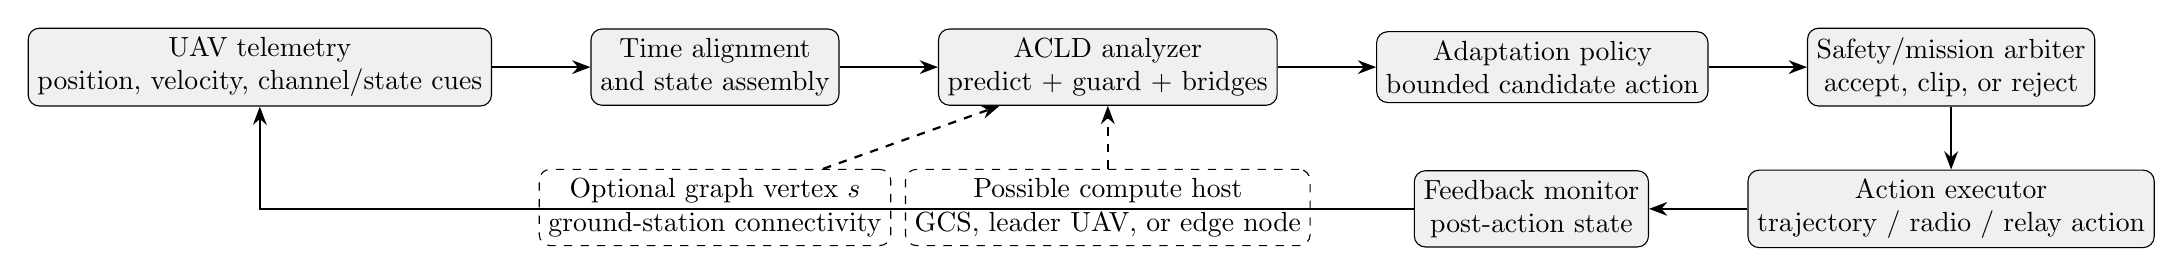
\begin{tikzpicture}[
      block/.style={rectangle,draw,rounded corners,align=center,minimum width=2.7cm,minimum height=0.9cm,fill=\ifcolor blue!8\else gray!12\fi},
      ext/.style={rectangle,draw,dashed,rounded corners,align=center,minimum width=2.7cm,minimum height=0.9cm},
      arrow/.style={-{Stealth},thick},
      node distance=0.8cm and 1.25cm
    ]
    \node[block] (telemetry) {UAV telemetry\\position, velocity, channel/state cues};
    \node[block, right=of telemetry] (align) {Time alignment\\and state assembly};
    \node[block, right=of align] (acld) {ACLD analyzer\\predict + guard + bridges};
    \node[block, right=of acld] (policy) {Adaptation policy\\bounded candidate action};
    \node[block, right=of policy] (safety) {Safety/mission arbiter\\accept, clip, or reject};
    \node[block, below=of safety] (execute) {Action executor\\trajectory / radio / relay action};
    \node[block, left=of execute] (feedback) {Feedback monitor\\post-action state};
    \node[ext, below=of align] (gsvertex) {Optional graph vertex $s$\\ground-station connectivity};
    \node[ext, below=of acld] (host) {Possible compute host\\GCS, leader UAV, or edge node};

    \draw[arrow] (telemetry) -- (align);
    \draw[arrow] (align) -- (acld);
    \draw[arrow] (acld) -- (policy);
    \draw[arrow] (policy) -- (safety);
    \draw[arrow] (safety) -- (execute);
    \draw[arrow] (execute) -- (feedback);
    \draw[arrow] (feedback.west) -| (telemetry.south);
    \draw[arrow,dashed] (gsvertex) -- (acld);
    \draw[arrow,dashed] (host) -- (acld);
  \end{tikzpicture}%
  }
  \caption{Deployment-level interpretation of ACLD. The optional ground-station vertex is part of the connectivity graph and is not synonymous with the host that executes the ACLD computation. The safety/mission arbiter remains authoritative over any mitigation action.}
  \label{fig:deployment_architecture}
\end{figure*}

\subsection{State acquisition and synchronization contract}
\label{subsec:state_contract}
At analysis time $t_k$, the reference implementation consumes a swarm-state object containing the kinematic and link-state features defined in Section~\ref{subsec:swarm_model}. The simulation provides kinematic and link-state features as a common-time snapshot. Transfer to a physical telemetry pipeline involves timestamped state acquisition, freshness limits, and handling of delayed or unavailable updates. Telemetry exchange and synchronization are external interfaces to the evaluated Python analyzer; packet-level latency and loss are addressed separately from the simulation core.

\subsection{Logical centralization and communication overhead}
\label{subsec:centralization_overhead}
Pairwise relations are formed from a global snapshot; the implementation is logically centralized rather than distributed. For $n$ UAVs, the compute-side pairwise geometry stage has $\mathcal O(n^2)$ candidate relations in the dense case. State-exchange traffic depends on the selected telemetry fields, update rate, serialization, transport, retransmission, and security overhead. The reported payload-only byte estimate provides a lower-bound traffic accounting; MAC/PHY overhead, retransmissions, and distributed synchronization depend on deployment-specific networking decisions.

\subsection{Adaptation and safety loop}
\label{subsec:adaptation_loop}
ACLD produces partition warnings, risky-link scores and forecast bridges. An autonomous deployment requires a separate policy for converting analyzer outputs into candidate actions, followed by a safety/mission arbiter that can accept, clip, delay, or reject the candidate. Separation of detection and control maintains the authority of collision avoidance, geofencing, energy constraints and mission priorities. The B1/B2 experiments quantify the outcome of one bounded heuristic intervention policy; controller optimization and full-architecture flight validation constitute separate evaluation targets. The resulting control interpretation is a closed loop:
\[
\text{Monitor}\rightarrow\text{Analyze}\rightarrow\text{Decide}\rightarrow\text{Safety Arbitrate}\rightarrow\text{Execute}\rightarrow\text{Monitor}.
\]

\section{Methodology: Adaptive Heuristic Framework for High-Mobility FANETs}
\label{sec:methodology}

The methodology formalizes the stochastic swarm model, derives adaptive distance thresholds, specifies a probabilistic channel model and details online partition-forecast and risk-cataloguing algorithms.  All symbols are declared once and used consistently; dimensional homogeneity is enforced throughout. Figure~\ref{fig:framework} depicts the full end-to-end pipeline, from state update to critical-link alert.

$\Delta t_{\text{ctrl}}$ denotes the controller/decision invocation period used in one-step prediction and in the finite-horizon analysis. $\Delta t_{\text{sim}}$ denotes the numerical simulation integration/logging step. The retained experiments use a 50-ms simulated decision step. The desktop core timing measurements and their relationship to the 50-ms simulated control period are reported in Section~\ref{subsec:runtime_analysis}. Unless otherwise stated, experiments use $\Delta t_{\text{ctrl}}=\Delta t_{\text{sim}}$.

\begin{figure}[ht]
  \centering
  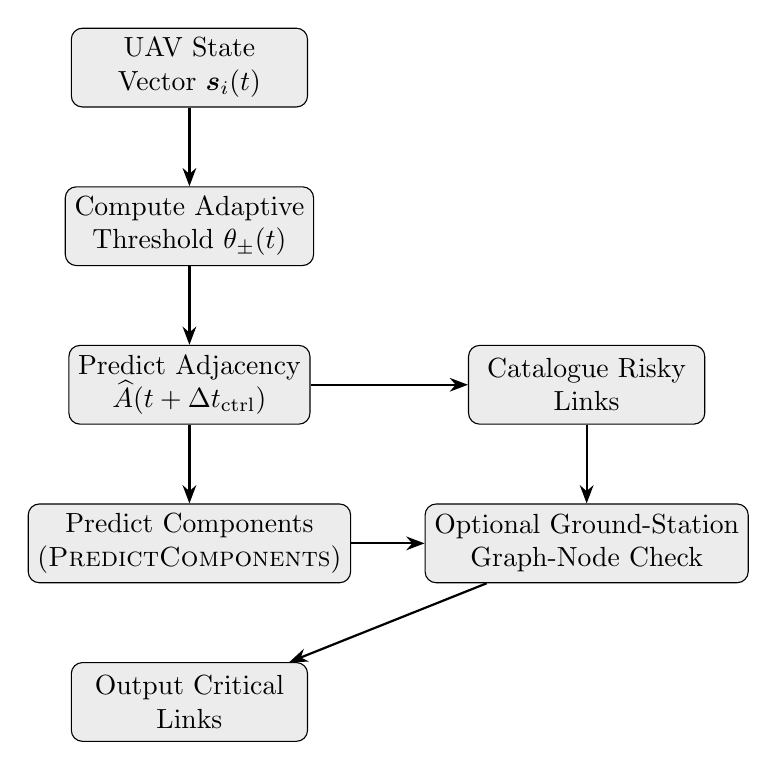
\begin{tikzpicture}[
      block/.style={
        rectangle, draw, rounded corners, align=center,
        fill=\ifcolor blue!10\else gray!15\fi, minimum width=3cm, minimum height=1cm
      },
      arrow/.style={-{Stealth}, thick},
      node distance=1cm and 2cm
    ]
    % Nodes
    \node[block] (state) {UAV State\\Vector $\boldsymbol s_i(t)$};
    \node[block, below=of state] (thr) {Compute Adaptive\\Threshold $\theta_\pm(t)$};
    \node[block, below=of thr] (pred) {Predict Adjacency\\$\widehat A(t+\Delta t_{\text{ctrl}})$};
    \node[block, below=of pred] (comp) {Predict Components\\(\textsc{PredictComponents})};
    \node[block, right=of pred] (risk) {Catalogue Risky\\Links};
    \node[block, below=of risk] (ground) {Optional Ground-Station\\Graph-Node Check};
    \node[block, below=of comp] (alert) {Output Critical\\Links};

    % Arrows
    \draw[arrow] (state) -- (thr);
    \draw[arrow] (thr) -- (pred);
    \draw[arrow] (pred) -- (comp);
    \draw[arrow] (pred) -- (risk);
    \draw[arrow] (comp) -- (ground);
    \draw[arrow] (risk) -- (ground);
    \draw[arrow] (ground) -- (alert);

  \end{tikzpicture}
  \caption{Adaptive critical link detection workflow.}
  \label{fig:framework}
\end{figure}

% ----------------------------------------------------------------------------
Figure~\ref{fig:risk_band_schematic} illustrates the risk-band bridge mechanism at graph level, without purporting to display UAV coordinates or a real S2 snapshot. \begin{figure}[htbp]
\centering
\SafeIncludeGraphics[width=.98\linewidth,keepaspectratio]{ACLD_BRIDGE_RISK_SCHEMATIC.pdf}
\caption{Conceptual example of inner-band components joined in the predicted viable graph by one risk-band bridge, followed by a possible next-step bridge loss. The node layout is schematic, not derived from the S2 trajectory coordinates; neither ACLD nor predictive Tarjan has a distinct bridge-localization advantage. The schematic provides no empirical evidence of controller action.}
\label{fig:risk_band_schematic}
\end{figure}

\subsection{Stochastic Swarm Dynamics with Connectivity Constraints}
\label{subsec:swarm_model}

Each UAV $u_i$ is represented at time $t$ by a controller-side feature vector
\[
  \boldsymbol s_i(t)=
  \bigl[\,
    \boldsymbol p_i^{\mathsf T}(t),
    \;\boldsymbol v_i^{\mathsf T}(t),
    \;\boldsymbol a_i^{\text{ctrl}\,\mathsf T}(t),
    \;\boldsymbol j_i^{\mathsf T}(t),
    \;h_i^{\text{ch}}(t),
    \;E_i(t)
  \bigr]^{\mathsf T}\!.
\]
The vector $\boldsymbol s_i(t)$ collects estimated/measured quantities and controller outputs used by the swarm logic.
Stochastic disturbances and sensor noise are modelled explicitly in the process/measurement equations rather than being
embedded in $\boldsymbol s_i(t)$.

Only the kinematic sub-state is filtered for estimation/simulation:
\[
  \boldsymbol x_i(t)=
  \bigl[\boldsymbol p_i^{\mathsf T}(t),\;\boldsymbol v_i^{\mathsf T}(t),\;\boldsymbol a_i^{\text{ctrl}\,\mathsf T}(t)\bigr]^{\mathsf T}
  \in \mathbb{R}^{9}.
\]
A discrete-time model is written as
\[
  \boldsymbol x_i(t+\Delta t_{\text{ctrl}})=f\!\bigl(\boldsymbol x_i(t)\bigr)+\boldsymbol\omega_i(t),
  \qquad
  \boldsymbol y_i(t)=h\!\bigl(\boldsymbol x_i(t)\bigr)+\boldsymbol\varepsilon_i(t),
\]
where $\boldsymbol\omega_i(t)\sim\mathcal N(\boldsymbol 0,\boldsymbol Q_{\mathrm{proc}})$ and
$\boldsymbol\varepsilon_i(t)\sim\mathcal N(\boldsymbol 0,\boldsymbol R_{\mathrm{KF}})$.
Wind gusts are treated as additive acceleration disturbances and absorbed into $\boldsymbol\omega_i(t)$.

\smallskip
\noindent\textit{Process covariance.}
\[
  \boldsymbol Q_{\mathrm{proc}}
  = \operatorname{diag}\!\bigl(\sigma_p^2\boldsymbol I_3,\;\sigma_v^2\boldsymbol I_3,\;\sigma_a^2\boldsymbol I_3\bigr)
  \in\mathbb{R}^{9\times 9},
\]
consistent with Section~\ref{subsec:sim_setup}.

\begin{description}[labelindent=0pt,leftmargin=0.85cm,font=\normalfont\itshape]

\item[\textbf{Position} $\boldsymbol p_i(t)\in\mathbb{R}^{3}$ (\si{\meter}):]
ENU-frame position estimate obtained from RTK-GNSS/VIO fusion (typical RMS $\le\SI{5}{\centi\meter}$) \cite{qin2018IEEE}.

\item[\textbf{Velocity} $\boldsymbol v_i(t)\in\mathbb{R}^{3}$ (\si{\meter\per\second}):]
Estimated linear velocity (e.g., IMU + GNSS Doppler fusion); bounded by $\lVert\boldsymbol v_i\rVert \le v_{\max}=\SI{23}{\meter\per\second}$ \cite{chen2008Ionospheric}.

\item[\textbf{Control acceleration} $\boldsymbol a_i^{\text{ctrl}}(t)\in\mathbb{R}^{3}$ (\si{\meter\per\square\second}):]
Desired translational acceleration command; bounded by $\lVert\boldsymbol a_i^{\text{ctrl}}\rVert \le a_{\max}\approx\SI{60}{\meter\per\square\second}$ \cite{mellinger2011IEEE}.

\item[\textbf{Jerk} $\boldsymbol j_i(t)\in\mathbb R^{3}$ (\si{\meter\per\cubic\second}):]
Discrete-time derivative of the commanded acceleration,
\[
  \boldsymbol j_i(t)=\frac{\boldsymbol a_i^{\text{ctrl}}(t)-\boldsymbol a_i^{\text{ctrl}}(t-\Delta t_{\text{ctrl}})}{\Delta t_{\text{ctrl}}}
\]
\cite{mellinger2011IEEE}.

\item[\textbf{Channel quality} $h_i^{\text{ch}}(t)\in\mathbb{R}$ (\si{\decibel}):]
Link-budget headroom derived from radio/telemetry feedback (for example RSSI, PER, selected MCS, or an equivalent link-quality estimate). The simulator uses channel-quality estimates exclusively through the probabilistic viability model; routing and MAC protocols are not emulated.

\item[\textbf{Remaining energy} $E_i(t)$ (\si{\joule}):]
$E_i(t)\in[0,E_{\max}]$ is the battery energy state.
The energy dynamics follow
\[
  \dot E_i(t)=-
  \bigl(P_i^{\text{prop}}(t)+P_i^{\text{comm}}(t)+P_i^{\text{payload}}(t)\bigr).
\]
A low-energy alarm is raised at $E_i(t)=E_{\min}=0.15\,E_{\max}$ \cite{zeng2016IEEE}.


\end{description}

\paragraph{Distances.}
The Euclidean separation between UAVs $i$ and $j$ is
\begin{equation}
  d^{\text{air}}_{ij}(t)=\|\boldsymbol p_i(t)-\boldsymbol p_j(t)\|_2,
  \qquad 1\le i<j\le n,
  \label{eq:distance_ij}
\end{equation}
where $n=|\mathcal V|$ is the number of UAVs. For brevity, $d_{ij}(t)\equiv d^{\text{air}}_{ij}(t)$ is used throughout.
The Laplacian-based network formulation follows the standard consensus literature \cite{olfati2007consensus}.


\subsubsection{Weighted Interaction Graph}
\label{subsubsec:weighted_graph}

The instantaneous communication topology is modeled as a time--varying, \emph{undirected} and \emph{symmetric} weighted graph
\(
  \mathcal G(t)=\bigl(\mathcal V,\mathcal E(t),w(t)\bigr)
\)
constructed in two steps.

\paragraph{Geometric candidates vs.\ channel-viable neighbours.}
Let $p_{\min}\in(0,1)$ be the minimum acceptable link-up probability.
Let $s_{ij}(t)\in[0,1]$ denote the link-up probability on $(i,j)$ at time $t$
(Section~\ref{subsec:prob_link_validation} gives $s_{ij}(t)=\Pr[\mathrm{SNR}_{ij}(t)\ge\gamma_0]$,
or $\Pr[\mathrm{SINR}_{ij}(t)\ge\gamma_0]$ under jamming).

Define the purely geometric candidate neighbour set
\[
  \mathcal N_i^{\mathrm{geo}}(t)
  = \bigl\{\,k \in \mathcal V\setminus\{i\}\ \big|\ d^{\text{air}}_{ik}(t)\le \theta_{ik,+}(t)\,\bigr\},
\]
and the \emph{viable} neighbour set (geometry + probability guard)
\[
  \mathcal N_i(t)
  = \bigl\{\,k \in \mathcal N_i^{\mathrm{geo}}(t)\ \big|\ s_{ik}(t)\ge p_{\min}\,\bigr\}.
\]

Accordingly, define the geometric candidate graph
$\mathcal G_{\mathrm{geo}}(t)=(\mathcal V,\mathcal E_{\mathrm{geo}}(t))$ with
$\mathcal E_{\mathrm{geo}}(t)=\{(i,j): j\in\mathcal N_i^{\mathrm{geo}}(t)\ \lor\ i\in\mathcal N_j^{\mathrm{geo}}(t)\}$,
and the channel-viable graph
$\mathcal G_{\mathrm{viable}}(t)=(\mathcal V,\mathcal E_{\mathrm{viable}}(t))$ with
$\mathcal E_{\mathrm{viable}}(t)=\{(i,j): j\in\mathcal N_i(t)\ \lor\ i\in\mathcal N_j(t)\}$.
Unless explicitly stated, the Laplacian in the subsection is built on $\mathcal G_{\mathrm{viable}}(t)$.

\paragraph{(i) Row-stochastic directed weights.}
Let the \emph{active neighbour set} be the channel-viable set (distance band + probability guard):
\[
  \mathcal N_i(t)
  = \bigl\{\,k \in \mathcal V\setminus\{i\}\ \big|\ d^{\text{air}}_{ik}(t)\le \theta_{ik,+}(t)\ \land\ s_{ik}(t)\ge p_{\min}\,\bigr\}.
\]

For every ordered pair \((i,j)\) define the directed weight
\begin{equation}
\begin{aligned}
  \tilde w_{ij}(t)&=
  \begin{cases}
    \dfrac{d^{\text{air}}_{ij}(t)^{-2}}
          {\displaystyle\sum_{k\in\mathcal N_i(t)} d^{\text{air}}_{ik}(t)^{-2}}, &
      j\in\mathcal N_i(t),\; i\neq j,\; |\mathcal N_i(t)|>0,\\[6pt]
    0, & \text{otherwise},
  \end{cases}\\[4pt]
  \sum_{j}\tilde w_{ij}(t)&=
  \begin{cases}
    1, & |\mathcal N_i(t)|>0,\\
    0, & |\mathcal N_i(t)|=0.
  \end{cases}
\end{aligned}
  \label{eq:w_tilde}
\end{equation}
Because numerator and denominator share the same \(\text{m}^{-2}\) units,
\(\tilde w_{ij}(t)\) is dimensionless.  
If a vertex is \emph{isolated} \(\bigl(|\mathcal N_i(t)|=0\bigr)\),
then \(\lambda_2\bigl(\boldsymbol L(t)\bigr)=0\) and ACLD raises a
partition alert at the next control cycle.

\paragraph{(ii) Symmetrisation.}
A real-symmetric Laplacian is obtained by averaging reciprocal
directed weights:
\begin{equation}
  w_{ij}(t)=\frac{\tilde w_{ij}(t)+\tilde w_{ji}(t)}{2},
  \qquad
  w_{ii}(t)=0,
  \label{eq:weights}
\end{equation}
so that \(w_{ij}=w_{ji}\ge 0\) for all \(i\neq j\).
Define the in-degree
\[
  \degIn{i}= \left| \left\{\, j \mid \tilde w_{ji}(t)>0\, \right\} \right|.
\]
Note that \(\sum_{j}\tilde w_{ij}(t)=1\) if \(|\mathcal N_i(t)|>0\) and
\(\sum_{j}\tilde w_{ji}(t)\le \degIn{i}\).
Hence
\[
  0\le\sum_{j} w_{ij}(t)
  =\tfrac12\!\Bigl(
      \sum_{j}\tilde w_{ij}(t)
    + \sum_{j}\tilde w_{ji}(t)
  \Bigr)
  \le \tfrac12\bigl(1+\degIn{i}\bigr).
\]

\[
  \boldsymbol D(t)=\operatorname{diag}\!\Bigl(\sum_{j}w_{ij}(t)\Bigr),\quad
  \boldsymbol W(t)=\bigl[w_{ij}(t)\bigr]_{i,j=1}^{n},\quad
  \boldsymbol L(t)=\boldsymbol D(t)-\boldsymbol W(t).
\]

Let \(\mathcal E(t)=\{(i,j) \mid w_{ij}(t)>0\}\) denote the instantaneous edge set.

\paragraph{Connectivity metric.}
Because \(\boldsymbol L(t)\) is symmetric and positive semidefinite,
the Laplacian eigenvalues satisfy \(0=\lambda_1\le\lambda_2\le\cdots\le\lambda_n\).
The \emph{algebraic connectivity}
\(\lambda_2\bigl(\boldsymbol L(t)\bigr)\) is strictly positive
iff \(\mathcal G(t)\) is connected~\cite{mesbahi2010graph}.  Let
\begin{equation}
  w_{\min}(t)=
  \begin{cases}
    \displaystyle
    \min_{\substack{i\neq j\\ w_{ij}(t)>0}} w_{ij}(t), & \mathcal E(t)\neq\varnothing,\\[6pt]
    0, & \text{otherwise},
  \end{cases}
  \label{eq:wmin}
\end{equation}
be the smallest positive off-diagonal weight. The minimum positive edge weight supports comparisons between local edge weights and spectral connectivity metrics,
although Theorem~\ref{thm:conn} is proved via a spanning-tree outage argument and does not explicitly require $w_{\min}(t)$.

% ---- INSERT right after Eq.~\ref{eq:wmin} ----
\paragraph*{Standing assumption (collision-avoidance safety buffer).} There exists a minimum inter--UAV separation $d_{\mathrm{safe}}>0$
enforced by the collision--avoidance layer; in particular, for every \emph{active} pair $(i,k)$ and time $t$ the following condition holds:
$d_{ik}(t)\ge d_{\mathrm{safe}}$. For design feasibility, the risk band is chosen so that $d_{\mathrm{safe}}<\theta_{ik,+}(t)$ for all admissible pairs, ensuring that at least one neighbour can exist under nominal conditions.

\begin{lemma}[Geometric weight floor under a safety buffer]
\label{lem:geom_floor}
Assume a collision-avoidance safety buffer $d_{\mathrm{safe}}>0$ such that
$d_{ik}(t)\ge d_{\mathrm{safe}}$ for every active pair $(i,k)$ at time $t$.
For $j\in\mathcal N_i(t)$ (implying $d_{ij}(t)\le \theta_{ij,+}(t)$) and 
$|\mathcal N_i(t)|>0$, then the directed weight satisfies
\[
  \tilde w_{ij}(t)
  \;=\;
  \frac{d_{ij}(t)^{-2}}{\sum_{k\in\mathcal N_i(t)} d_{ik}(t)^{-2}}
  \;\ge\;
  \Bigl(\tfrac{d_{\mathrm{safe}}}{\theta_{ij,+}(t)}\Bigr)^{\!2}
  \frac{1}{|\mathcal N_i(t)|}.
\]
Moreover, for the symmetrised weight $w_{ij}(t)=\tfrac12(\tilde w_{ij}(t)+\tilde w_{ji}(t))$ the following condition holds:
\[
  \resizebox{0.98\linewidth}{!}{$\displaystyle w_{ij}(t)\;\ge\;\tfrac12\max\!\left\{
    \mathbb{I}\{j\in\mathcal N_i(t)\}\Bigl(\tfrac{d_{\mathrm{safe}}}{\theta_{ij,+}(t)}\Bigr)^{\!2}\frac{1}{|\mathcal N_i(t)|},
    \;
    \mathbb{I}\{i\in\mathcal N_j(t)\}\Bigl(\tfrac{d_{\mathrm{safe}}}{\theta_{ji,+}(t)}\Bigr)^{\!2}\frac{1}{|\mathcal N_j(t)|}
  \right\}.$}
\]
\end{lemma}

\begin{proof}
Since $j\in\mathcal N_i(t)$ implies $d_{ij}(t)\le \theta_{ij,+}(t)$ and $x\mapsto x^{-2}$ is decreasing,
the monotonicity of inverse-square distance implies $d_{ij}(t)^{-2}\ge \theta_{ij,+}(t)^{-2}$.
For the denominator, the safety buffer yields $d_{ik}(t)\ge d_{\mathrm{safe}}$ for all $k\in\mathcal N_i(t)$,
hence $d_{ik}(t)^{-2}\le d_{\mathrm{safe}}^{-2}$ and therefore
$\sum_{k\in\mathcal N_i(t)} d_{ik}(t)^{-2}\le |\mathcal N_i(t)|\,d_{\mathrm{safe}}^{-2}$.
Combining both bounds gives
\[
\tilde w_{ij}(t)\ge
\frac{\theta_{ij,+}(t)^{-2}}{|\mathcal N_i(t)|\,d_{\mathrm{safe}}^{-2}}
=
\Bigl(\tfrac{d_{\mathrm{safe}}}{\theta_{ij,+}(t)}\Bigr)^{\!2}
\frac{1}{|\mathcal N_i(t)|}.
\]
Finally, $w_{ij}(t)=\tfrac12(\tilde w_{ij}(t)+\tilde w_{ji}(t))\ge \tfrac12\max\{\tilde w_{ij}(t),\tilde w_{ji}(t)\}$,
and substituting the directed lower bounds yields the stated inequality.
\end{proof}


\begin{corollary}[A safe lower bound for $w_{\min}(t)$]
\label{cor:wmin_floor}
Define, for each unordered pair $(i,j)$,
\[
  \resizebox{0.98\linewidth}{!}{$\displaystyle \psi_{ij}(t)=\max\!\left\{
    \mathbb{I}\{j\in\mathcal N_i(t)\}\Bigl(\tfrac{d_{\mathrm{safe}}}{\theta_{ij,+}(t)}\Bigr)^{\!2}\frac{1}{|\mathcal N_i(t)|},
    \;
    \mathbb{I}\{i\in\mathcal N_j(t)\}\Bigl(\tfrac{d_{\mathrm{safe}}}{\theta_{ji,+}(t)}\Bigr)^{\!2}\frac{1}{|\mathcal N_j(t)|}
  \right\}.$}
\]
Then, for the symmetrised graph,
\[
  w_{\min}(t)\;\ge\;\tfrac12\min_{(i,j)\,:\,w_{ij}(t)>0}\,\psi_{ij}(t).
\]
\end{corollary}

\medskip\noindent
\textbf{Important remark.}
All proofs that rely on the row-stochastic property must work with the \emph{directed} matrix \(\tilde{\boldsymbol W}(t)\).  The symmetrised \(\boldsymbol W(t)\) loses that property but guarantees \(\boldsymbol L(t)=\boldsymbol L(t)^\top\), enabling spectral analysis.

% ---------------------------------------------------------------------------
% Optional ground-station graph vertex
% ---------------------------------------------------------------------------
\subsubsection{Optional Ground-Station Connectivity Node}
\label{subsubsec:central}

When infrastructure connectivity is part of the scenario, a fixed ground-station \emph{graph vertex} \(s\) at position \(\boldsymbol p_s\) may be appended to the swarm graph, extending the vertex set to \(\mathcal V'=\mathcal V\cup\{s\}\) with cardinality \(n'=n+1\). The ground-station augmentation is optional: UAV-only connectivity is obtained by omitting \(s\). Importantly, the graph vertex \(s\) is not the definition of the ACLD compute host; Section~\ref{sec:system_architecture} treats compute placement separately. Throughout the subsection, all augmented matrices carry a prime (e.g., \(\boldsymbol L'(t)\in\mathbb R^{n'\times n'}\)); the prime is dropped again in later sections once the dimensions are clear.

\paragraph{Unified distance.}
\begin{equation}
  d^{\text{mix}}_{ik}(t)=
  \begin{cases}
    d^{\text{air}}_{ik}(t), & k\neq s,\\[4pt]
    d^{\text{gs}}_{is}(t),  & k=s.
  \end{cases}
  \label{eq:dmix}
\end{equation}

\paragraph{Row-stochastic directed weights.}
Let the UAV-only neighbour set be the channel-viable set $\mathcal N_i(t)$ defined in Section~\ref{subsubsec:weighted_graph}.

Define the augmented set
\[
  \mathcal N_i'(t)
  = \mathcal N_i(t)\ \cup\
    \bigl\{\,s\ \big|\ d^{\text{gs}}_{is}(t)\le\theta_{is,+}(t)\ \land\ s_{is}(t)\ge p_{\min}\,\bigr\}.
\]

For \(k\in\mathcal N_i'(t)\) set
\[
  \tilde w_{ik}(t)=
  \frac{ \bigl[d^{\text{mix}}_{ik}(t)\bigr]^{-2}}
       {\displaystyle
        \sum_{\ell\in\mathcal N_i'(t)}
        \bigl[d^{\text{mix}}_{i\ell}(t)\bigr]^{-2}},
  \qquad
  \sum_{k}\tilde w_{ik}(t)=
  \begin{cases}
    1, & |\mathcal N_i'(t)|>0,\\
    0, & |\mathcal N_i'(t)|=0.
  \end{cases}
\]
\emph{Isolated UAV.} If \(|\mathcal N_i'(t)|=0\) then
\(\tilde w_{ik}(t)\equiv 0\) for all \(k\).

For the ground station,
\[
\begin{aligned}
  \tilde w_{si}(t)&=
  \begin{cases}
    \dfrac{{\bigl[d^{\text{gs}}_{is}(t)\bigr]^{-2}}}
           {\displaystyle\sum_{j\in\mathcal N_s(t)}
           {\bigl[d^{\text{gs}}_{js}(t)\bigr]^{-2}}}, &
      |\mathcal N_s(t)|>0,\\[6pt]
    0, & |\mathcal N_s(t)|=0,
  \end{cases}\\[4pt]
  \mathcal N_s(t)&=
  \bigl\{\,i\ \big|\ d^{\text{gs}}_{is}(t)\le\theta_{is,+}(t)\ \land\ s_{is}(t)\ge p_{\min}\,\bigr\}.
\end{aligned}
\]

\paragraph{Symmetrisation (extends Eq.~\ref{eq:weights}).}
\[
  w_{ik}(t)=\frac{\tilde w_{ik}(t)+\tilde w_{ki}(t)}{2},
  \qquad
  w_{ii}(t)=0,
\]
yielding a real-symmetric weight matrix \(\boldsymbol W'(t)\) and a symmetric Laplacian \(\boldsymbol L'(t)=\boldsymbol D'(t)-\boldsymbol W'(t)\)
at all times.  Proofs that rely on row-stochastic properties (e.g., Theorem~\ref{thm:conn}) must use the directed matrix \(\tilde{\boldsymbol W}'(t)\), not the symmetrised \(\boldsymbol W'(t)\).

Note that $\sum_{k}\tilde w_{ik}(t)=1$ whenever $|\mathcal N_i'(t)|>0$, preserving row-stochasticity.
% ---------------------------------------------------------------------------
% 3.2.3 Adaptive Distance Threshold
% ---------------------------------------------------------------------------
\subsection{Adaptive Distance Threshold}
A baseline communication range $\mathrm{cthr}_{\text{base}}$ is modulated to
account for dispersion, relative motion, and attitude divergence:
\begin{equation}
\begin{aligned}
  \mathrm{cthr}_{ij}(t)
  ={}&\mathrm{cthr}_{\text{base}}\Biggl[
     1
     + \alpha\,\frac{\sigma_d(t)}{\bar d(t)}
     - \beta\,\frac{\|\boldsymbol v_i-\boldsymbol v_j\|_2}{2v_{\max}}\\
     &\hspace{2.8em}- \gamma\,\frac{\Delta\theta_{ij}(t)}{\pi}
     - \delta\,\frac{\|\boldsymbol a^{\text{ctrl}}_i-\boldsymbol a^{\text{ctrl}}_j\|_2}{2a_{\max}}
     - \zeta\,\frac{\|\boldsymbol j_i-\boldsymbol j_j\|_2}{2j_{\max}}
   \Biggr],
\end{aligned}
  \label{eq:cthradp}
\end{equation}
where
\begin{itemize}[nosep]
  \item $\mathrm{cthr}_{\text{base}}$ is the nominal communication range,
  \item $\alpha,\beta,\gamma,\delta,\zeta$ are dimensionless gains  
        (\(\alpha,\beta,\gamma\in[0,1)\); \(\delta,\zeta\in[0,0.2]\) by default),
  \item $\sigma_d(t)$ and $\bar d(t)$ are the standard deviation and mean of all link distances $\{d^{\text{air}}_{ij}(t)\}$,
  \item $\|\boldsymbol v_i(t)-\boldsymbol v_j(t)\|_2$ is the relative speed,
  \item $v_{\max}$ is the maximum UAV speed,
  \item $\Delta\theta_{ij}(t)$ is the absolute heading‐angle difference,
  \item $\|\boldsymbol a^{\text{ctrl}}_i(t)-\boldsymbol a^{\text{ctrl}}_j(t)\|_2$ is the relative control acceleration,
  \item $a_{\max}$ is the maximum feasible acceleration,
  \item $\|\boldsymbol j_i(t)-\boldsymbol j_j(t)\|_2$ is the relative jerk,
  \item $j_{\max}$ is the maximum feasible jerk.
\end{itemize}

\paragraph{UAV--ground-station adaptive threshold.}
For the fixed ground station $s$, the heading-difference term is undefined and is omitted.
Define, for each UAV $i$,
\begin{equation}
 \mathrm{cthr}_{is}(t)
  =\mathrm{cthr}_{\text{base}}
   \Bigl[
     1 
     + \alpha\,\frac{\sigma_d(t)}{\bar d(t)}
     - \beta\,\frac{\|\boldsymbol v_i(t)\|_2}{v_{\max}}
     - \delta\,\frac{\|\boldsymbol a^{\text{ctrl}}_i(t)\|_2}{a_{\max}}
     - \zeta\,\frac{\|\boldsymbol j_i(t)\|_2}{j_{\max}}
   \Bigr],
  \label{eq:cthradp_gs}
\end{equation}
and set the UAV--GS risk bands as
\[
  \theta_{is,-}(t)=0.97\,\mathrm{cthr}_{is}(t),\qquad
  \theta_{is,+}(t)=\mathrm{cthr}_{is}(t).
\]

Risk bands then follow:
\begin{equation}
  \theta_{ij,-}(t)=0.97\,\mathrm{cthr}_{ij}(t),\qquad
  \theta_{ij,+}(t)=\mathrm{cthr}_{ij}(t).
  \label{eq:risk_bands}
\end{equation}

The factor \(0.97\) defines the conservative inner band used throughout the main evaluation; inner-band margin sensitivity is discussed in Section~\ref{subsec:param_validation}.

\paragraph{Symmetry of UAV--UAV thresholds.}
For any UAV pair $(i,j)$, the terms in~\eqref{eq:cthradp} are symmetric:
$\|\boldsymbol v_i-\boldsymbol v_j\|_2=\|\boldsymbol v_j-\boldsymbol v_i\|_2$,
$\|\boldsymbol a_i^{\text{ctrl}}-\boldsymbol a_j^{\text{ctrl}}\|_2=\|\boldsymbol a_j^{\text{ctrl}}-\boldsymbol a_i^{\text{ctrl}}\|_2$,
$\|\boldsymbol j_i-\boldsymbol j_j\|_2=\|\boldsymbol j_j-\boldsymbol j_i\|_2$,
and $\Delta\theta_{ij}(t)=\Delta\theta_{ji}(t)$ by definition.
Hence $\mathrm{cthr}_{ij}(t)=\mathrm{cthr}_{ji}(t)$ and $\theta_{ij,\pm}(t)=\theta_{ji,\pm}(t)$ for UAV--UAV links.
No symmetry is assumed/required for UAV--ground-station links.


% ---------------------------------------------------------------------------
% Parameter Tuning and Selected Values
% ---------------------------------------------------------------------------
\subsection{Parameter Tuning and Selected Values}
\label{subsec:parameter_values}

The evaluated ACLD parameter configuration is
\[
  \alpha = 0.00,\qquad
  \beta = 0.10,\qquad
  \gamma = 0.20,\qquad
  \delta = 0.10,\qquad
  \zeta = 0.05,
\]
with inner-band fraction
\[
  \theta_{ij,-}(t)=0.97\,\mathrm{cthr}_{ij}(t),
  \qquad
  \theta_{is,-}(t)=0.97\,\mathrm{cthr}_{is}(t).
\]

The stated coefficients define the operating point evaluated by the implementation and the available campaigns using exact next-step bridge ground truth. Ablation effects are assessed using the corresponding experiment records rather than inferred from coefficient values.

Unless otherwise stated, the reported results use the stated parameter set with the channel model of Section~\ref{subsec:prob_link_validation} and the protocol of Section~\ref{sec:simulation}.

\subsection{Probabilistic Link Validation}
\label{subsec:prob_link_validation}
Under Nakagami‐$m$ fading, the probability of meeting SNR target~$\gamma_0$ on link~$(i,j)$ is
\begin{equation}
  \Pr[\mathrm{SNR}_{ij}\ge\gamma_0] =
  \frac{\Gamma\!\bigl(m,\,m\,\frac{\gamma_0}{\overline{\mathrm{SNR}}_{ij}(t)}\bigr)}
       {\Gamma(m)}
  \label{eq:pr_snr}
\end{equation}

where
\begin{itemize}[nosep]
  \item $m>0$ is the Nakagami fading parameter,
  \item $\Gamma(\cdot,\cdot)$ is the upper incomplete gamma function,
  \item $d_0$ is the reference distance,
  \item $\plExp$ is the path‐loss exponent (typically $2\le\plExp\le4$),
  \item $\overline{\mathrm{SNR}}_0$ is the average \emph{linear} SNR (i.e.\ dB values are converted via $10^{\mathrm{dB}/10}$) at reference distance $d_0$,
\end{itemize}

The evaluated channel stresses include receiver-referenced jamming. Joint jamming/spoofing and field-measured channels represent complementary test conditions.

\paragraph{Success and outage probabilities (notation used throughout).}
Define the link success probability
\[
  s_{ij}(t) := \Pr\!\big[\mathrm{SNR}_{ij}(t)\ge \gamma_0\big]
\]
(and under jamming, replace SNR by SINR accordingly), and the outage probability
\[
  p^{\mathrm{out}}_{ij}(t) := 1 - s_{ij}(t).
\]
The viability/guard condition is
\[
  s_{ij}(t)\ge p_{\min}
  \quad \Longleftrightarrow \quad
  p^{\mathrm{out}}_{ij}(t)\le 1-p_{\min}.
\]
In the theorem, \(p_{\max}\) is a post-mitigation outage cap enforced on selected spanning-tree edges.


\paragraph{Jamming-aware SINR (receiver-referenced JNR).}
Let $B$ denote the signal bandwidth and $\NF$ the receiver noise figure (dB).
Define the effective noise-floor power in bandwidth $B$ as
\[
  \NB\;[\mathrm{dBm}] = -174 + 10\log_{10}(B\;[\mathrm{Hz}]) + \NF .
\]
Let $P^{\mathrm{rx}}_{J,i}(t)$ be the received jammer power at receiver $i$ in \si{\deci\bel m} and define
\[
\JNR_i(t)\;[\mathrm{dB}] := P^{\mathrm{rx}}_{J,i}(t)\;[\mathrm{dBm}] - \NB\;[\mathrm{dBm}],
  \qquad
  j_{\mathrm{lin},i}(t) := 10^{\JNR_i(t)/10}.
\]
For a link $(i,j)$ use a conservative link-level interference ratio
\[
  j_{\mathrm{lin},ij}(t) := \max\{j_{\mathrm{lin},i}(t), j_{\mathrm{lin},j}(t)\}.
\]
Then the average SINR at distance $d_{ij}(t)$ is
\[
  \overline{\mathrm{SINR}}_{ij}(t)=
  \frac{\overline{\mathrm{SNR}}_0\,(d_0/d_{ij}(t))^{\plExp}}{1+j_{\mathrm{lin},ij}(t)},
\]
and the Nakagami-$m$ success probability becomes
\[
  \Pr[\mathrm{SINR}_{ij}\ge\gamma_0] =
  \frac{\Gamma\!\bigl(m,\,m(\gamma_0/\overline{\mathrm{SINR}}_{ij}(t))\bigr)}{\Gamma(m)}.
\]
The calculated success probability enters the viability test with threshold $p_{\min}$.


\subsubsection*{Channel–Model Parameterisation}

Table~\ref{tab:nakagami_params} lists the numerical settings adopted for Nakagami-$m$ fading and path-loss calculations.  
Unless otherwise stated, the \emph{default UAV--UAV link} (last row) defines the baseline simulation profile. Sensitivity conclusions are restricted to the available simulation sweep outputs.

\begin{table}[H]
  \centering
  \caption{Illustrative channel parameters used by the sub-6 GHz link abstraction.}
  \label{tab:nakagami_params}
  \renewcommand{\arraystretch}{1.15}
  \begin{tabular}{@{}lllll@{}}
    \toprule
    \textbf{Scenario} & $m$ & $\overline{\mathrm{SNR}}_0$ [dB] & $d_0$ [m] & $\plExp$ \\
    \midrule
    Free-space LoS (rural)   & 3–4 & 25 & 100 & 2.0 \\
    Suburban NLoS            & 2   & 20 & 100 & 2.6–2.8 \\
    Urban LoS (macro)        & 2–3 & 22 & 100 & 2.2–2.5 \\
    Urban NLoS (canyon)      & 1–2 & 15 & 100 & 3.0–3.5 \\
    \textbf{Default UAV–UAV*}& \textbf{2.5} & \textbf{22} & \textbf{100} & \textbf{2.4} \\
    \bottomrule
  \end{tabular}
  \vspace{-0.35em}
  \begin{minipage}{0.9\linewidth}\footnotesize
    \emph{*Simulation profile for small multirotor UAV links. The channel layer is technology-agnostic and does not constitute an IEEE 802.11s protocol emulation or a field measurement. UAV--ground-station links use the Free-space LoS parameter row when the optional ground-station vertex is enabled.}
  \end{minipage}
\end{table}

The simulated LoS/NLoS profiles represent an illustrative channel parameter sweep informed by published standards. Reported sensitivity effects derive from the retained simulations; protocol-level measurements and field-calibrated propagation are separate validation layers.

%============================================================
\subsection{Connectivity‐Preservation Theorem}
\label{subsec:connectivity_theorem}

The connectivity theorem characterizes a higher-level mitigation policy under explicit spanning-tree feasibility and conditional edge-outage assumptions. The B1/B2 heuristic-control experiments measure a separate, concrete implementation and are interpreted according to their observed outcomes.

\begin{definition}[Guaranteed/viable edge sets and ACLD alarm set]
\label{def:edge_sets}
Fix a slot index $k$ with $t_k=t_0+k\Delta t_{\text{ctrl}}$.

\emph{Current guaranteed (inner-band) edge set} at the measurement time $t_k$:
\[
  \mathcal E_-^{\mathrm{cur}}(t_k)
  :=
  \left\{(i,j): d_{ij}(t_k)\le \theta_{ij,-}(t_k)\ \land\ s_{ij}(t_k)\ge p_{\min}\right\}.
\]

Let the one-step kinematic forecast be
$\widehat{\boldsymbol p}_i=\boldsymbol p_i(t_k)+\boldsymbol v_i(t_k)\Delta t_{\text{ctrl}}$
and $\widehat d_{ij}=\|\widehat{\boldsymbol p}_i-\widehat{\boldsymbol p}_j\|_2$.
Define the predicted success probability (evaluate~\eqref{eq:pr_snr} by substituting $d_{ij}\leftarrow \widehat d_{ij}$):
\[
  \widehat s_{ij}(t_{k+1}\mid t_k) := \Pr\!\big[\mathrm{SNR}_{ij}(t_{k+1})\ge \gamma_0\ \big|\ \widehat d_{ij}\big]
  \quad (\text{or SINR under jamming}).
\]

\emph{Predicted guaranteed edges} (used by Algorithms~\ref{alg:kneighbors}--\ref{alg:components}):
\[
  \widehat{\mathcal E}_-(t_{k+1}\mid t_k)
  :=
  \left\{(i,j): \widehat d_{ij}\le \theta_{ij,-}(t_k)\ \land\ \widehat s_{ij}(t_{k+1}\mid t_k)\ge p_{\min}\right\}.
\]

\emph{Predicted viable (outer-band) edges}:
\[
  \mathcal E_+(t_{k+1}\mid t_k)
  :=
  \left\{(i,j): \widehat d_{ij}\le \theta_{ij,+}(t_k)\ \land\ \widehat s_{ij}(t_{k+1}\mid t_k)\ge p_{\min}\right\}.
\]

\emph{Predicted risk-band edges (used for alarms)}:
\[
  \mathcal E_{\mathrm{risk}}(t_k)
  := \mathcal E_+(t_{k+1}\mid t_k)\setminus \widehat{\mathcal E}_-(t_{k+1}\mid t_k).
\]

ACLD outputs an \emph{alarm set} $\mathcal R(t_k)\subseteq \mathcal E_{\mathrm{risk}}(t_k)$ by
(i) predicting components on $\widehat{\mathcal E}_-(t_{k+1}\mid t_k)$ via Algorithm~\ref{alg:components} and
(ii) cataloguing risky inter-component links via Algorithms~\ref{alg:risky} and~\ref{alg:ground}. Define the predicted viable graph $\mathcal G_+(t_{k+1}\mid t_k) := (\mathcal V, \mathcal E_+(t_{k+1}\mid t_k))$.
\end{definition}

\begin{definition}[ACLD-respecting controller policy]
\label{def:acld_policy}
A higher-level controller policy $\pi$ is \emph{ACLD-respecting} if the policy receives, at each slot $t_k$,
$\mathcal R(t_k)$ and applies a bounded mitigation action on a selected subset of alarmed links,
using either:
\begin{enumerate}[label=(\alph*),leftmargin=1.0cm]
\item \textbf{Tx-power bump:} increase transmit power (or coding/MCS margin) on $(i,j)$ by $\Delta P_{ij}(t_k)\in[0,\Delta P_{\max}]$,
thereby increasing the average link budget and reducing outage; and/or
\item \textbf{Micro-trajectory tweak:} add a bounded relative motion correction so that the next-slot separation decreases by at least
$\Delta d_{ij}(t_k)\in[0,\Delta d_{\max}]$ without violating the collision-avoidance buffer $d_{\mathrm{safe}}$.
\end{enumerate}
The minimal policy acts only on alarmed links required for spanning-tree preservation.
\end{definition}

\begin{assumption}[Policy-enforced band-gap and per-tree outage cap]
\label{asm:policy_bandgap}
Let $\pi$ be an ACLD-respecting controller. At each slot $t_k$, the controller selects a spanning tree $T(t_k)$ of the \emph{current guaranteed} graph $\mathcal G_-^{\mathrm{cur}}(t_k)$ whenever the graph is connected. Whenever ACLD raises alarms on edges that are needed to preserve $T(t_k)$ for the next slot, the controller applies a bounded mitigation action such that:

\begin{enumerate}[label=(\roman*),leftmargin=1.0cm]
\item \textbf{Band-gap (tree preservation):} $T(t_k)\subseteq \mathcal E_+(t_{k+1}\mid t_k)$.
\item \textbf{Uniform per-tree outage cap:} every tree edge $e=(i,j)\in T(t_k)$ satisfies
$p^{\mathrm{out}}_{ij}(t_{k+1})\le p_{\max}$ after mitigation, for some constant $p_{\max}\in(0,1)$ with $(|\mathcal{V}|-1)p_{\max}<1$.
\end{enumerate}

The assumed policy property has not been established for the B1/B2 heuristic. For a multi-step bound, the feasibility and outage conditions must hold conditional on every preceding successful-connectivity history, rather than merely on an unconditional averaged sample.
\end{assumption}

\begin{assumption}[Conditional tree feasibility across slots]
\label{asm:conditional_tree_feasible}
For each slot $k=0,\ldots,M-1$, conditional on the full observation/control history and on connectivity having survived through slot $k$, the current guaranteed inner-band graph has a spanning tree $T(t_k)$; the tree satisfies the next-slot viability inclusion after policy action, and every selected tree edge has a conditional next-slot outage probability no larger than $p_{\max}$. The stochastic graph and real channel must obey the same conditional outage bounds. Uniform feasibility and outage conditions are assumptions rather than inferences from the B1/B2 data.
\end{assumption}

\begin{theorem}[Finite-horizon exponential lower bound on connectivity]
\label{thm:conn}
Let $t_0\ge 0$ and suppose $\lambda_2(\boldsymbol L(t_0))\ge \underline{\lambda}>0$. 
Under Assumptions~\ref{asm:policy_bandgap} and~\ref{asm:conditional_tree_feasible},
with per-history conditional per-edge outage bounded by $p^{\mathrm{out}}_{ij}(t)\le p_{\max}$ for every selected tree edge,
and with $(|\mathcal{V}|-1)p_{\max}<1$, the following bound holds for $T=M\Delta t_{\text{ctrl}}$:
\[
  \Pr\!\Bigl[\min_{0\le k\le M}\lambda_2\bigl(\boldsymbol L(t_0+k\Delta t_{\text{ctrl}})\bigr)>0\Bigr]
  \;\ge\; \exp\!\bigl(-\kappa\,T\bigr),
\]
where
\[
  \kappa = \frac{(|\mathcal{V}|-1)\,p_{\max}}{\bigl(1-(|\mathcal{V}|-1)p_{\max}\bigr)\,\Delta t_{\text{ctrl}}}.
\]
\end{theorem}

\begin{proof}[Proof of Theorem~\ref{thm:conn}]
The identity $\lambda_2(\boldsymbol L(t))>0 \Leftrightarrow \mathcal G(t)$ connected is standard.

\textit{Step 1 — One-step tree preservation via policy-enforced band-gap.}
By Assumptions~\ref{asm:policy_bandgap} and~\ref{asm:conditional_tree_feasible}, on each surviving connectivity history the controller selects a spanning tree $T(t_k)$ from the guaranteed graph
and, when ACLD raises alarms on edges needed to preserve that tree, applies bounded mitigation.
The inclusion $T(t_k)\subseteq \mathcal E_+(t_{k+1}\mid t_k)$ follows from the assumed band-gap condition rather than from the implemented ACLD decision rule.
Absent fading outages, $\mathcal G_+(t_{k+1}\mid t_k)$ is connected.

\textit{Step 2 — Single-step disconnection bound under fading.}
A necessary condition for disconnection at $t_{k+1}$ is that at least one edge of the preserved spanning tree $T(t_k)$ experiences outage: if every tree edge remains available, the preserved spanning tree certifies graph connectivity. Therefore the disconnection event is contained in the union of the tree-edge outage events, and the union bound gives
\[
  \Pr[\text{disconnect at }t_{k+1}] \;\le\; |T(t_k)|\,p_{\max} \;=\; (|\mathcal{V}|-1)\,p_{\max}
  \;\doteq\; q_{\max} \;<\;1,
\]
where $|\mathcal{V}|$ is the total number of nodes in the considered topology (including the ground station, if present).

\textit{Step 3 — Product bound and exponential lower bound.}
Using the chain rule and the uniform \emph{conditional} per-slot bound (not independence of adaptive graph states), the probability of no disconnection across $M$ consecutive slots is at least
\[
  (1-q_{\max})^{M} \;\ge\; \exp\!\Bigl(-\tfrac{q_{\max}}{1-q_{\max}}\,M\Bigr),
\]
where $\ln(1-x)\ge -x/(1-x)$ for $x\in(0,1)$ is used. With $T=M\Delta t_{\text{ctrl}}$ and $q_{\max}=(|\mathcal{V}|-1)p_{\max}$, the stated bound follows with
\(
  \kappa = \frac{(|\mathcal{V}|-1)p_{\max}}{\bigl(1-(|\mathcal{V}|-1)p_{\max}\bigr)\,\Delta t_{\text{ctrl}}}.
\)
\end{proof}

\noindent\textbf{Non-vacuity note.} The bound requires $(|\mathcal V|-1)p_{\max}<1$. For example, with 1,000 UAVs and a ground-station node, the condition requires $p_{\max}<0.001$ for each selected tree edge on every surviving history. The implemented viability threshold $p_{\min}=0.90$ does not independently establish a post-mitigation conditional bound; hence no non-vacuous large-swarm bound has been demonstrated. The spanning-tree preservation requirement is explicitly assumed and is not proved from the implemented controller.\par
\noindent\textbf{Interpretation and scope.} The bound is conditional on a controller preserving a suitable spanning tree, the current guaranteed graph admitting such a tree on every surviving history, and a per-edge conditional outage cap holding at every step. The B1/B2 heuristic experiments do not verify that the assumptions hold, so the theorem is not an empirical connectivity guarantee for ACLD. The one-step probabilistic viability model also does not establish packet-level or hardware deployment reliability.


\subsection{Predicted Adjacency Matrix}
\label{subsec:prediction}

\begin{remark}[Threshold drift]
If risk-band separation weakens within a slot, tree inclusion can fail. A Lipschitz perturbation bound $\|\boldsymbol L(t_{k+1})-\boldsymbol L(t_k)\|_2\le L\Delta t_{\mathrm{ctrl}}$ and Weyl's inequality imply one-step connectivity only when $\lambda_2(\boldsymbol L(t_k))>L\Delta t_{\mathrm{ctrl}}$. No multistep exponential guarantee follows from the perturbation bound alone. The theorem therefore relies on the explicit conditional spanning-tree feasibility and outage assumptions rather than an unspecified inflation of $\kappa$.
\end{remark}

Forecast positions at $t+\Delta t_{\text{ctrl}}$ are
$\widehat{\boldsymbol p}_i=\boldsymbol p_i(t)+\boldsymbol v_i(t)\Delta t_{\text{ctrl}}$.  A link $(i,j)$ is \emph{viable} if
\begin{equation}
  \widehat d_{ij}\le\theta_{ij,+}(t)
  \quad\text{and}\quad
  \Pr\bigl[\text{SNR}_{ij}\ge\gamma_0\bigr]\ge p_{\min},
\end{equation}
where
\begin{itemize}[nosep]
  \item $\widehat d_{ij}=\|\widehat{\boldsymbol p}_i-\widehat{\boldsymbol p}_j\|_2$,
  \item $p_{\min}\in[0,1]$ is the minimum acceptable link‐up probability.
\end{itemize}

Thus the predicted adjacency is
\[
   \widehat A_{ij}(t+\Delta t_{\text{ctrl}})
   =\begin{cases}1,&\text{if viable},\\0,&\text{otherwise.}\end{cases}
\]

% ----------------------------------------------------------------------------
\subsection{Pseudocode for Online Algorithms}
\label{subsec:pseudocode}

\noindent\textbf{Notation:} Node indices start at zero.  Assume:
\begin{itemize}[nosep]
  \item $\widehat A$ is symmetric (i.e. $\widehat A = \max(\widehat A,\widehat A^\top)$).  
  \item $\widehat d_{ij}$ stores predicted distances from $\widehat p_i = p_i + v_i\,\Delta t_{\text{ctrl}}$.  
  \item Pairwise thresholds $\theta_{ij,-}(t),\theta_{ij,+}(t)$ are precomputed.
\end{itemize}

% .................................. Algorithm 1 ............................
\paragraph{$k$-Hop Neighborhood Exploration.}
Algorithm~\ref{alg:kneighbors} finds all nodes reachable from a seed node $i$. By setting the hop limit $k_{\max} = n_{\text{total}}$, the routine operates as a full Breadth-First Search (BFS) to guarantee complete discovery of connected components.

\begin{algorithm}[H]\small
  \caption{\textsc{KNeighbors} (depth-limited BFS on guaranteed edges)}
  \label{alg:kneighbors}
  \begin{algorithmic}[1]
    \Require{adjacency list $adj$, $\widehat d$, $\theta_-$; seed node $i$; hop limit $k_{\max}$}    
    \Ensure{$C$ — nodes reachable from $i$ within $k_{\max}$ hops using edges with $\widehat d\le\theta_-$}
    \State $Seen \gets \{i\}$; Queue $Q \gets [(i,0)]$
    \While{$Q \neq []$}
      \State pop $(u,depth)$ from $Q$
      \If{$depth = k_{\max}$} \State \textbf{continue} \EndIf
      \ForAll{$v \in adj[u]$}
        \If{$\widehat d_{uv}\le\theta_{uv,-}$ \textbf{and} $v\notin Seen$}
          \State add $v$ to $Seen$; push $(v,depth+1)$ into $Q$
        \EndIf
      \EndFor
    \EndWhile
    \State \Return $Seen$
  \end{algorithmic}
\end{algorithm}
% .................................. Algorithm 2 ............................
\paragraph{Component Prediction.}
Algorithm~\ref{alg:components} partitions all vertices into predicted connected components by repeated $k$-hop exploration.

\begin{algorithm}[H]\small
  \caption{\textsc{PredictComponents}}
  \label{alg:components}
  \begin{algorithmic}[1]
    \Require{adjacency list $adj$, $\widehat d$, $\theta_-$; hop limit $k_{\max}$; number of vertices $n_{total}$}
    \Ensure{$\mathcal C = \{C_1,\dots,C_q\}$ — list of components}
    \State $Unseen \gets \{0,1,\dots,n_{total}-1\}$; $\mathcal C \gets []$;
    \While{$Unseen \neq \emptyset$}
      \State pick $i \in Unseen$;
      \State $C \gets$ \textsc{KNeighbors}($adj, \widehat d, \theta_- ,\,i,\,k_{\max}$);
      \State append $C$ to $\mathcal C$;
      \State $Unseen \gets Unseen \setminus C$;
    \EndWhile
    \State \Return $\mathcal C$;
  \end{algorithmic}
\end{algorithm}
% .................................. Algorithm 3 ............................
\paragraph{Risky Link Cataloging.}
Algorithm~\ref{alg:risky} classifies each active link in the risk band $(\theta_-,\theta_+]$ as inter- or intra-component risky.

\begin{algorithm}[H]\small
  \caption{\textsc{CatalogueRiskyLinks}}
  \label{alg:risky}
  \begin{algorithmic}[1]
    \Require{$\mathcal C,\;\widehat A,\;\widehat d,\;\theta_-,\theta_+$}
    \Ensure{$\mathcal R_{\mathrm{inter}},\;\mathcal R_{\mathrm{intra}}$}
    \State build map $compOf[u] = index$ for each $u$ in component $\mathcal C$
    \State $\mathcal R_{\mathrm{inter}} \gets []$; $\mathcal R_{\mathrm{intra}} \gets []$;
    \ForAll{pairs $(i,j)$ with $i<j$ and $\widehat A_{ij}=1$}
      \If{$\theta_{ij,-}<\widehat d_{ij}$} \Comment{$\widehat A_{ij}=1$ already implies $\le\theta_{ij,+}$}
        \If{$compOf[i] \neq compOf[j]$}
          \State append $(i,j)$ to $\mathcal R_{\mathrm{inter}}$;
        \Else
          \State append $(i,j)$ to $\mathcal R_{\mathrm{intra}}$;
        \EndIf
      \EndIf
    \EndFor
    \State \Return $\mathcal R_{\mathrm{inter}},\;\mathcal R_{\mathrm{intra}}$;
  \end{algorithmic}
\end{algorithm}
% .................................. Algorithm 4 ............................
\paragraph{Separation of Ground-Related Risky Links.}
Algorithm~\ref{alg:ground} filters $\mathcal R_{\mathrm{inter}}$, separating $s$–UAV vs.\ UAV–UAV risky links in $\mathcal O(r)$ time.

\newcommand{\sDashUAV}{\text{s\textendash UAV}}
\newcommand{\dashUAV}{\text{UAV\textendash UAV}}

\begin{algorithm}[H]\small
  \caption{\textsc{SeparateGroundLinks} ($\mathcal O(r)$ separation)}
  \label{alg:ground}
  \begin{algorithmic}[1]
    \Require{inter-risky links $\mathcal R_{\mathrm{inter}}$, central index $s$}
    \Ensure{$\mathcal R_{\sDashUAV},\;\mathcal R_{\dashUAV}$}
    \State $\mathcal R_{\sDashUAV}\gets []$; $\mathcal R_{\dashUAV}\gets []$
    \ForAll{$(i,j)\in \mathcal R_{\mathrm{inter}}$}
      \If{$i=s$ \textbf{or} $j=s$}
        \State append $(i,j)$ to $\mathcal R_{\sDashUAV}$
      \Else
        \State append $(i,j)$ to $\mathcal R_{\dashUAV}$
      \EndIf
    \EndFor
    \State \Return $\mathcal R_{\sDashUAV},\;\mathcal R_{\dashUAV}$
  \end{algorithmic}
\end{algorithm}

\subsection{Reference baselines and comparison protocol}
\label{subsec:baselines}

\paragraph{B0 — No-heuristic baseline (NH).} No proactive detection and no mitigation are applied. The swarm evolves only under mobility and the channel model; partition events are counted when $\lambda_2(\boldsymbol L(t)) < 10^{-3}$ (same threshold used throughout the paper). All percentage claims on “partition reduction” are reported relative to NH unless stated otherwise.

\paragraph{B1 — Tarjan-on-snapshot (TARJAN@t).} Run bridge/articulation detection~\cite{tarjan1972dfs} on $A(t)$; all bridges are flagged as risky. \emph{Pros:} $O(n{+}m)$. \emph{Cons:} Snapshot-only; ignores fading and the geometry at $t{+}\Delta t$.

\paragraph{B2 — Predict-then-Bridge (TARJAN@\texorpdfstring{$t{+}\Delta t_{\text{ctrl}}$}{t+dt\_ctrl}).} Use the kinematic forecast to build $\widehat{A}(t{+}\Delta t_{\text{ctrl}})$, then run Tarjan. \emph{Pros:} anticipates next-step topology. \emph{Cons:} still ignores channel uncertainty unless combined with a probability guard.

\paragraph{B3 — Edge-betweenness (EB-APPX).} Approximate edge betweenness (Brandes/sampling)~\cite{brandes2001betweenness}; pick top-$\eta$ edges as risky. \emph{Pros:} captures multi-path significance. \emph{Cons:} $O(nm)$ exact (unweighted); costly at scale, and snapshot-only.

\paragraph{B4 — Min-cut / $k$-edge connectivity (CUT/KEC).} Compute global min cut (e.g., Stoer–Wagner~\cite{stoer1997mincut}) or use $k$-edge connectivity proxies (e.g., Nagamochi–Ibaraki~\cite{nagamochi1992edgeconn}). \emph{Pros:} rigorous global connectivity view. \emph{Cons:} global property; not tailored to per-edge \emph{imminent} failure under dynamics/fading.

\paragraph{ACLD vs. baselines.}
The evaluation explicitly reports Tarjan-on-predicted-graph with the Nakagami guard, the geometry-only Tarjan variant, and an edge-betweenness baseline. CUT/KEC is retained as a conceptual reference point in the methodological discussion, but no corresponding results are included in the manuscript tables because no matched long-run CUT/KEC output is available.

\paragraph{Complexity summary.}
TARJAN is $O(n{+}m)$~\cite{tarjan1972dfs}; EB exact is $O(nm)$ (unweighted)~\cite{brandes2001betweenness}; CUT/KEC depends on routine (e.g., Stoer–Wagner $O(nm{+}n^2\log n)$~\cite{stoer1997mincut}).

% ----------------------------------------------------------------------------
\subsection{Complexity Analysis}
\label{subsec:complexity}
Let $n=|\mathcal V'|$ be the number of vertices, $m = \frac{1}{2}\|\widehat A\|_0$ the number of unique undirected edges in the predicted adjacency, $m_- = |\{(i,j):\widehat d_{ij}\le\theta_-(t)\}|$ the number of guaranteed links, and $r=|\mathcal R_{\mathrm{inter}}|$ the number of inter-component risky links. Table~\ref{tab:complexity} summarizes the worst-case time complexity of each stage in a single control cycle.

\begin{table}[H]
  \centering
  \caption{Time complexity of core routines per control cycle.}
  \label{tab:complexity}
  \renewcommand{\arraystretch}{1.2}
  \begin{tabular}{@{}ll@{}}
    \toprule
    \textbf{Stage} & \textbf{Time Complexity}\\
    \midrule
    Distance computation (pairwise)        & $\mathcal O(n^2)$\\
    Link-up probability calculation       & $\mathcal O(n^2)$\\
    Adaptive threshold computation        & $\mathcal O(n^2)$\\
    Predicted adjacency construction      & $\mathcal O(n^2)$\\
    \textsc{KNeighbors}                   & $\mathcal O(k\,m_-)$\\
    \textsc{PredictComponents}            & $\mathcal O(n + m_-)$\\
    \textsc{CatalogueRiskyLinks}          & $\mathcal O(m)$\\
    Build $adj$ for $\mathcal R_{\mathrm{inter}}$ & $\mathcal O(r)$\\
    \textsc{SeparateGroundLinks} (Linear scan)        & $\mathcal O(r)$\\
    \midrule
    Dense pair formation (lower-bound stage) & $\mathcal O(n^2)$\\
    \bottomrule
  \end{tabular}
\end{table}

\noindent\emph{Complexity qualification.} A quadratic pairwise construction stage is present, but a universal $\mathcal O(n^2)$ upper bound for every mode cannot be deduced from the stage-wise table when traversal depth $k$ grows with $n$. The C2 empirical log--log slope is descriptive and is not a worst-case proof.


\noindent\textit{Table note.} The parameter choices follow 3GPP TR 38.901~\cite{3gpp38901}
and ITU-R P.1411-10~\cite{itur1411}. The value $\overline{\mathrm{SNR}}_0$ is specified in dB
and converted to linear scale via $10^{\text{dB}/10}$ before being used in the probability
model~\eqref{eq:pr_snr}.
% ----------------------------------------------------------------------------

\paragraph{Evidence-bound manuscript tables.}
The validated results in Section~\ref{sec:simulation} use exact next-step bridge ground truth and distinguish warning from localization. Results from nonmatched exploratory timing runs are excluded from the inferential comparisons. Cross-method speed rankings are not inferred from noncomparable incremental timing scopes.

\subsection{Implementation Considerations}
\label{subsec:implementation}

The implementation is a Python notebook/script workflow using NumPy/SciPy-style kernels for geometry and graph operations. A separately logged audit environment used Python 3.14.3 with recorded dependency versions; historical campaign worker environments were not uniformly recorded. The measured C2 runtime pertains to the recorded non-isolated Windows host, and no portable latency statement follows. Monte-Carlo units can be executed in parallel, but repeated seed identifiers across scenarios create dependence that is retained in cluster-based inferential sensitivity analyses.

\begin{itemize}[leftmargin=*]
  \item \textbf{Parallelism}: Monte-Carlo units are amenable to campaign-level parallel execution, but seeds reused across scenarios are treated as common clusters. The historical worker-executed source fingerprints are incomplete; no unrecorded executor configuration is assumed.
  \item \textbf{Numerics}: Pairwise distances are computed in vectorized form (\texttt{numpy} broadcasting / \texttt{scipy.spatial.distance}) to avoid Python-level loops.
  \item \textbf{Timing methodology}: Runtime summaries report repeated wall-clock measurements from \texttt{time.perf\_counter()} and list the median, interquartile range, mean, and p95 for each $n$ in the standalone C2 benchmark.
  \item \textbf{Memory}: Peak memory footprint is $\mathcal{O}(n+m)$ for graph storage, with a dense distance stage of $\mathcal{O}(n^2)$ when the graph is fully connected.
\end{itemize}

% ----------------------------------------------------------------------------

\subsection{Summary}
\label{subsec:summary}
The predictive graph pipeline, warning policy, and conditional spanning-tree formulation establish the mathematical setting for the empirical evaluation in Section~\ref{sec:simulation}.
% ============================================================================
% End of Methodology
% ============================================================================

\section{Simulation and Results}
\label{sec:simulation}

\subsection{Protocol and metric definitions}
\label{subsec:baselines_metrics}
Reported outcomes derive from validated campaign records. Separate evaluation targets are (i) \emph{edge localization}, scored against the exact bridge set of the realized next-step viable graph; (ii) \emph{partition early warning}, a binary prediction of next-step graph disconnection; (iii) controller effects; and (iv) core computational cost. The temporal target is one control step (50 ms), not long-horizon link persistence. The predictive Tarjan reference uses the same forecast viable graph as ACLD. Snapshot Tarjan and edge-betweenness are additional structural comparators. Cut/edge-connectivity is discussed conceptually because there is no matched long-run export for a valid empirical cut-policy comparison.

The per-episode edge-localization score is the micro-aggregated quantity
\begin{equation}
 F1_{\mathrm{edge}}=\frac{2TP_{\mathrm{edge}}}{2TP_{\mathrm{edge}}+FP_{\mathrm{edge}}+FN_{\mathrm{edge}}},
\end{equation}
with counts summed over steps; no-support steps contribute zero counts, not a fabricated zero F1. Partition warning FPR is $FP/(FP+TN)$ and is undefined when an episode contains no negative steps. The recorded episode-mean implementation assigns zero to undefined-FPR episodes. Both the historical episode-mean convention and negative-support pooled alternatives are reported. Edge-localization and partition-warning scores use different prediction targets and denominators.

\subsection{Experimental setup and audit coverage}
\label{subsec:sim_setup}
The reference implementation uses synthetic mobility with a 0.05 s step, a 200 s episode horizon, bounded state predictions, and channel-viability thresholds. The dataset campaigns and recorded source provenance are summarized in Table~\ref{tab:campaign_coverage}. A1 contains 350 episode-method records from the P0.4-origin label-audited dataset and 2,350 records from the P0.5 dataset; A3 records originate from P0.5. The A1 and A3 records retain their historical P0.4/P0.5 provenance. A2, B1, B2, C1 and C3 carry P0.6 campaign metadata; historical worker-level executable fingerprints are characterized in Section~\ref{sec:reproducibility}.

\begin{table}[htbp]
\centering\small
\caption{Validated campaign record counts. B1/B2 rows are controller episodes; other episode rows are method observations.}
\label{tab:campaign_coverage}
\begin{tabular}{lrrl}\toprule
Campaign & Episode records & ACLD step records & Scope\\\midrule
A1 & 2700 & 2159460 & detection core\\
A2 & 3600 & 2879280 & Rician-condition detection\\
A3 & 240 & 239940 & ablation\\
B1 & 600 & 479880 & nominal closed loop\\
B2 & 600 & 479880 & stressed closed loop\\
C1 & 500 & 399900 & detection scaling\\
C3 & 480 & 639840 & ground-station sensitivity\\\bottomrule
\end{tabular}
\end{table}

\subsection{Forecast-bridge localization and risk-gated warning}
\label{subsec:param_validation}
In A2, 36 scenarios and 20 seeds yield 720 matched scenario--seed units, with five evaluated methods per unit. ACLD achieved mean episode edge micro-F1 0.99605 and PEW-F1 0.99958. Predictive Tarjan achieved exactly the same edge micro-F1 (0.99605), as both methods selected the same predicted viable-graph bridge set. The matched localization results identify the partition-warning decision rule as the distinguishing evaluated component of ACLD.

\begin{table}[htbp]
\centering\small
\caption{A2 matched comparison. FPR values use the documented episode-mean zero-negative-support convention unless stated as pooled.}
\label{tab:a2_comparison}
\begin{tabular}{lrrr}\toprule
Method & Edge micro-F1 & PEW-F1 & Episode-mean FPR\\\midrule
ACLD v3 & 0.99605 & 0.99958 & 0.03097\\
Predictive Tarjan & 0.99605 & 0.99782 & 0.24175\\\bottomrule
\end{tabular}
\end{table}

Of the 720 A2 units, 151 episodes have no negative warning-label support. Across the genuinely negative steps (59,607 in total), ACLD yielded 2,304 false positives and predictive Tarjan 12,180. The respective \emph{pooled} FPRs were 0.03865 and 0.20434, respectively, a relative reduction of about 81.08\%. Under the recorded episode-mean convention the relative reduction is 87.19\%. Episode-mean and pooled FPR estimates have different denominators and cannot be used interchangeably. Across the fixed 73-scenario A1/A2/C1 grid, scenario-balanced ACLD-minus-Tarjan FPR had a mean difference of -0.21840 (scenario-bootstrap 95\% interval [-0.26414,-0.17572]); reused seed clusters limit a simple independent-scenarios interpretation. A conservative test family also assigns $p=1$ to the structurally identical edge-localization scores.

\begin{figure}[htbp]\centering
\SafeIncludeGraphics[width=.78\linewidth,height=.27\textheight,keepaspectratio]{detection_metrics.png}
\caption{Detection metrics from the recorded simulation campaigns. Edge localization and binary partition warnings evaluate different targets.}
\label{fig:audited_detection}
\end{figure}

\paragraph{Why identical localization and different false alarms coexist.}
The implemented ACLD edge selection is the sorted unique set of predicted viable bridges, the same edge set returned by predictive Tarjan. ACLD applies an additional risk-gated binary warning condition involving disconnection, a small spectral gap, or predicted bridges jointly with intercomponent risk. Predictive Tarjan warns on disconnection or any predicted bridge. Thus identical bridge TP/FP/FN totals can coexist with markedly different binary-warning false positives.

\input{S1_warning_rule_addendum.tex}
\input{S2_MANUSCRIPT_INSERT_EN.tex}

\subsection{Retrospective S2 onset-warning analysis}\label{subsec:s2_onset}
S2 partition labels include persistent disconnections and newly developing partitions, so full-label scores do not isolate warnings preceding a new loss of connectivity. A \emph{retrospective} onset analysis reused all 40 saved S2 paired unit files, fixed labels and source manifests. The onset-specific definition was developed after inspection of the S2 results; the retrospective analysis is not a new simulation campaign or a preregistered independent confirmation. The current graph is classified as connected when the saved \texttt{lambda2\_current} exceeds $10^{-10}$, matching the S4 numerical criterion. For a saved step $t$, define the onset indicator
\begin{equation}
 Y_t^{\mathrm{onset}}=\mathbb{I}[\lambda_2(L_t)>10^{-10}]\,\mathbb{I}[Y_{t+1}^{\mathrm{partition}}=1].
\label{eq:onset}
\end{equation}
The \emph{at-risk population} contains only currently connected steps; a true negative is a currently connected step followed by a connected next-step graph. The labels are graph-connectivity labels in the synthetic simulator, not measured packet delivery or independent physical failures.

There were 3,096 currently connected steps and 156,864 already disconnected steps among 159,960 S2 transitions; the at-risk set contains 46 new partition events and 3,050 negative cases. Table~\ref{tab:s2_onset} recomputes decision outcomes only within that at-risk set, explicitly distinguishing warning false-positive rate (FPR), recall and precision. The components-only variant is obtained from the saved predicted viable component count and uses the same frozen graph state, not a newly tuned model.
\begin{table}[htbp]
\centering\small
\caption{Post-hoc S2 new-partition onset evaluation restricted to currently connected graph states. Forty scenario--seed units share 10 distinct seed identifiers; time steps are temporally dependent.}
\label{tab:s2_onset}
\begin{tabular}{@{}lrrrrr@{}}\toprule
Warning rule & TP & FN & FP & FPR (\%) & Precision (\%)\\\midrule
ACLD risk gate & 45 & 1 & 117 & 3.84 & 27.78\\
Predictive Tarjan & 46 & 0 & 712 & 23.34 & 6.07\\
Components only & 40 & 6 & 4 & 0.13 & 90.91\\\bottomrule
\end{tabular}
\end{table}
\begin{figure}[htbp]
\centering
\SafeIncludeGraphics[width=.97\linewidth,keepaspectratio]{S2_ONSET_RULE_COMPARISON_EN.pdf}
\caption{Retrospective, post-hoc S2 onset-only comparison of pooled false-positive rate (left) and recall (right), conditioned on the network being connected at decision time. Forty scenario--seed units share 10 distinct seed IDs; the denominator for the false-positive rate is 3,050 at-risk negatives and recall has 46 new partitions. Error bars are not shown because adjacent time steps are not independent. The explicit bootstrap difference is reported in the text.}
\label{fig:onset_rule_comparison}
\end{figure}

\begin{figure}[htbp]
\centering
\SafeIncludeGraphics[width=.97\linewidth,keepaspectratio]{S2_WARNING_TIMELINE_EN.pdf}
\caption{Illustrative real S2 decision trace for the fixed source unit with 150 UAVs, medium/NoJam, seed 252 (decision times 0--7.05 s). Filled squares denote emitted alarms while the current graph is connected; diamonds mark realized next-step partition onsets (at 4.30, 5.55 and 5.95 s). Current-disconnected intervals are omitted, and the example is not a representative-sample performance estimator. The graph and label sequences are unchanged from the archived CSV.}
\label{fig:onset_timeline}
\end{figure}

ACLD's onset recall is $45/46=97.83\%$ (Tarjan: $46/46=100\%$; components only: $40/46=86.96\%$). Against predictive Tarjan, the ACLD-onset FPR difference is $-19.51$ percentage points. An exploratory 5,000-replicate percentile bootstrap resampling \emph{entire seed clusters} across the four scenario strata yielded a conditional 95\% interval of $[-23.85,-15.36]$ percentage points for that pooled-FPR difference. The conditional interval does not represent independent-time-step uncertainty and does not support transfer to other channel models or real UAV operations. The 46 onset events share only 10 S2 seed clusters under fixed scenario strata.

The operational ranking depends on the cost assigned to a missed new partition relative to an unnecessary alert. Components-only minimized observed false alarms but missed six new onsets; predictive Tarjan missed none but generated 712 false alerts, whereas ACLD occupied an intermediate point with one miss and 117 false alerts. The full-label S2 counts (122 versus 718 false positives) use a \emph{different} negative population including post-disconnection transitions. Both evaluations are retained, with onset metrics emphasized for pre-failure warning (Fig.~\ref{fig:onset_rule_comparison}); a fixed, archival decision trace illustrates the corresponding time structure (Fig.~\ref{fig:onset_timeline}). The S2 CSVs, per-unit onset summary, Python verification script and seed-block bootstrap code are included in the accompanying reproducibility materials.


\subsection{Ablation, Rician approximation, and ranking limits}
\label{subsec:robustness}
In A3, full ACLD attained mean edge F1 of 0.99516. Removing the forecast-bridge component yielded 0.10734; removing the guard produced 0.74519, while the no-adaptive-threshold variant yielded 0.69350. Ablation results characterize the roles of forecast bridges, viability guarding, and adaptive thresholds within the evaluated graph task; the matched predictive-Tarjan comparison characterizes edge-selection equivalence. Top-1 recall remains sensitive to the number of true bridges because only a single ranked edge is evaluated against a potentially larger reference set.

A2's Rician parameters are specified in dB and mapped to the moment-matched Nakagami shape via $K_{\mathrm{lin}}=10^{K_{\mathrm{dB}}/10}$ and $m=(K_{\mathrm{lin}}+1)^2/(2K_{\mathrm{lin}}+1)$. The moment-matching formula yields $m=1.33333$ at $K=0$ dB and $m=1.79773$ at $K=3$ dB. The channel model evaluates deterministic success probabilities without sampling instantaneous Rician fading. For the recorded NoJam settings, the viability guard is nonbinding within the 100 m geometric range, explaining exact nominal graph/decision equivalence. Jammed conditions can activate the guard. Nominal parameter equivalence provides no universal fading-robustness guarantee.

\begin{figure}[htbp]\centering
\SafeIncludeGraphics[width=.78\linewidth,height=.27\textheight,keepaspectratio]{rician_sensitivity.png}
\caption{Scenario-conditional Rician-to-Nakagami sensitivity; equivalent NoJam outputs reflect the nonbinding probability threshold.}
\label{fig:rician_audited}
\end{figure}

The supplementary material contains the top-$k$ edge-localization diagnostic (Supplementary Figure S1), without changing the matched predictive-Tarjan result.

\subsection{Closed-loop controller study}
\label{subsec:closedloop}
The B1/B2 controller experiments quantify the connected-fraction effect of coupling the warning analyzer to a bounded heuristic intervention. Mean connected fractions for ACLD and no intervention (NH) were respectively 0.031916 and 0.030049 in B1, and 0.005733 and 0.005272 in B2. The corresponding absolute improvements are approximately 0.187 and 0.046 percentage points. In B2, ACLD and predictive Tarjan had identical mean connected fractions under the tested controller. Consequently, the closed-loop results cannot independently justify a broad claim of robust sustained connectivity or a large incremental control advantage.

\begin{table}[htbp]
\centering\small
\caption{Connected fraction in closed-loop evaluation. Values are proportions, not percentages.}
\label{tab:closedloop_support}
\begin{tabular}{lrrr}\toprule
Campaign & No intervention & ACLD controller & Gain (pp)\\\midrule
B1 nominal & 0.030049 & 0.031916 & 0.187\\
B2 stress & 0.005272 & 0.005733 & 0.046\\\bottomrule
\end{tabular}
\end{table}

\begin{figure}[htbp]\centering
\SafeIncludeGraphics[width=.78\linewidth,height=.27\textheight,keepaspectratio]{closed_loop_performance.png}
\caption{Small closed-loop connected-fraction effects; the vertical axis and denominators must be read explicitly.}
\label{fig:closedloop_audited}
\end{figure}

\subsection{Core runtime, scaling, and communication estimate}
\label{subsec:runtime_analysis}
The checkpointed serial C2 benchmark completed 1000 measurements at each of $n\in\{50,150,300,500,1000\}$ UAVs (5000 unique measurements). The timer covers \texttt{ACLDCore.run\_acld(state)} only, excluding kinematics, I/O, telemetry synchronization, and baseline shared preprocessing. Table~\ref{tab:runtime_audited} gives the observed desktop results. Median duration exceeds the 50-ms controller period from 150 UAVs onward under the measured conditions, providing no evidence of large-swarm real-time feasibility.

\begin{table}[htbp]
\centering\small
\caption{Serial C2 core execution times on the recorded non-isolated Windows machine (ms; 1000 repeats per size).}
\label{tab:runtime_audited}
\begin{tabular}{rrrr}\toprule
UAVs & Median & Mean & 95th percentile\\\midrule
50 & 10.976 & 10.988 & 12.674\\
150 & 58.015 & 58.728 & 65.964\\
300 & 244.406 & 246.465 & 278.963\\
500 & 828.972 & 834.996 & 997.966\\
1000 & 3751.072 & 3796.560 & 4638.740\\\bottomrule
\end{tabular}
\end{table}

\begin{figure}[htbp]\centering
\SafeIncludeGraphics[width=.78\linewidth,height=.27\textheight,keepaspectratio]{runtime_scaling.png}
\caption{Measured core runtime by UAV count. Interquartile range and 95th percentile describe measurement spread, not parameter uncertainty or portable performance.}
\label{fig:runtime_audited}
\end{figure}

Mean monitored system CPU utilization during the C2 benchmark was approximately 80.2\%. A five-size log--log fit gave a descriptive slope of 1.965 ($R^2=0.9908$); the measured slope does not establish asymptotic complexity. The existing C4 calculation assumes 14 float32 state scalars per UAV, yielding 56 payload bytes per UAV per 50 ms cycle. The payload estimate excludes headers, control signaling, contention, routing, retries and security overhead; no packet-trace measurement was performed.

\subsection{Probability mapping, denominator checks, and reliability limits}
\label{subsec:calibration}
The recorded bounded warning score is a heuristic, not an estimated probability; raw-score reliability and Brier-type calculations are therefore only diagnostics. A separately authorized sigmoid mapping was fitted on A1/A2 seeds 42--51 and evaluated without refitting on disjoint A1/A2 seeds 52--61 and the independent C1 seed family. Aggregate Brier/ECE values were respectively 0.00017518/0.00019931 on the A1/A2 holdout and 0.00018627/0.00013788 on C1. Small aggregate errors do \emph{not} establish uniform calibration.

The A1/A2 holdout bin with mean mapped probability 0.4504 had observed event frequency 0.0469 among 512 temporally dependent steps; the corresponding C1 bin had frequency 0.1000 among 40 steps. A finer score-level analysis found probability 0.9398 paired with observed frequencies 0.0606 (132 steps) and 0.0500 (20 steps), respectively. Only three of ten fixed probability bins contained observations in each evaluation split. Sparse-bin discrepancies constrain calibration claims; assessment after additional model fitting requires a separate validation split.

\begin{figure}[htbp]\centering
\SafeIncludeGraphics[width=.78\linewidth,height=.27\textheight,keepaspectratio]{approved_sigmoid_reliability.png}
\caption{Reliability diagnostics of the separately fitted sigmoid mapping. Sparse-bin deviations are not resolved by a low global ECE.}
\label{fig:sigmoid_reliability}
\end{figure}

\input{S3_MANUSCRIPT_INSERT_EN.tex}
\subsection{Interpretation and scope of evidence}
\label{subsec:discussion_audited}
The main measured contribution is a risk-gated partition-warning rule operating on forecast bridges also identified by matched predictive Tarjan. In the retrospective S2 onset population, ACLD detected 45 of 46 new partitions with 117 false alarms, compared with 46 detections and 712 false alarms for predictive Tarjan. The components-only rule traded a further reduction in false alarms for six missed onsets. Figures~\ref{fig:onset_rule_comparison} and~\ref{fig:onset_timeline} show the onset-conditioned decision analysis and one explicitly identified archived trajectory. The warning-policy trade-off is the relevant performance endpoint; predicted bridge localization remains equivalent to the matched comparator. The spectral and component alarms coincided in A2 and S2.\par

The empirical scope comprises synchronized synthetic swarm states, a 50-ms next-step graph-connectivity target, and a moment-matched channel-viability abstraction. The onset analysis reduces the influence of already disconnected states on evaluation, while seed-cluster resampling accounts for reuse of seed identifiers across scenario strata. The B1/B2 controller effects, core runtime, and sigmoid reliability measurements are separately quantified in Sections~\ref{subsec:closedloop}, \ref{subsec:runtime_analysis}, and \ref{subsec:calibration}. Transfer to operational FANETs motivates additional studies with asynchronous telemetry, packet-level traces, optimized execution, and field-calibrated radio models. Conditional spanning-tree requirements and historical source provenance are documented separately in Sections~\ref{subsec:s4_theorem_evidence} and~\ref{sec:reproducibility}.\par

\subsection{S4: Conditional connectivity bound and observed open-loop topology}\label{subsec:s4_theorem_evidence}
Theorem~\ref{thm:conn} establishes a connectivity bound for a policy satisfying conditional spanning-tree and outage constraints. The S2 open-loop records characterize actual graph connectivity, including time to first partition. Post-action spanning-tree selection and history-conditional edge outages form distinct measurements needed to assess the theorem assumptions for a particular controller.

All 40 S2 scenario--seed units (10 unique seeds reused across four scenario strata) began with an observed connected graph (current algebraic connectivity above a numerical tolerance of $10^{-10}$). For all 40 units a partition appeared before the end of the 200-s simulated horizon; no unit remained continuously connected throughout the 3,999 future-transition labels per unit. Across the 159,960 observed current states, 3,096 were connected (1.9355\%). The current algebraic-connectivity status at $t_{k+1}$ agreed with the realized next-step partition label recorded at $t_k$ for all 159,920 temporally paired comparisons. The median time to first partition was 2.975 s and 2.875 s for 50-UAV medium/NoJam and dense/J15 conditions, and 4.600 s for both 150-UAV conditions (10 seeds per condition). The open-loop topology results provide a baseline description of first-partition timing rather than a post-mitigation controller trial.

\begin{table}[htbp]
\centering\small
\caption{S4 open-loop continuity of the observed current graph; 10 S2 seeds per condition (seed IDs reused across conditions).}
\label{tab:s4_survival}
\begin{tabular}{lrrr}\toprule
Condition & \shortstack{Connected\\at start} & \shortstack{Uninterrupted\\200 s} & \shortstack{Median first\\split (s)}\\\midrule
50 UAV, medium/NoJam & 10/10 & 0/10 & 2.975\\
50 UAV, dense/J15 & 10/10 & 0/10 & 2.875\\
150 UAV, medium/NoJam & 10/10 & 0/10 & 4.600\\
150 UAV, dense/J15 & 10/10 & 0/10 & 4.600\\\bottomrule
\end{tabular}
\end{table}

\begin{figure}[htbp]
\centering
\includegraphics[width=.78\linewidth,height=.27\textheight,keepaspectratio]{S4_uninterrupted_connectivity_survival.png}
\caption{Uninterrupted connected-state survival in S2, starting from connected observed graphs. Curves track the first realized partition and are not post-mitigation survival probabilities.}
\label{fig:s4_survival}
\end{figure}

The guard $p_{\min}=0.90$ yields only an individual model-based outage upper bound of 0.10 for accepted edges. For a tree over $N$ vertices, the theorem requires $q=(N-1)p_{\max}<1$, so $p_{\max}<1/(N-1)$. With an optional ground-station vertex, the bound requires caps strictly below 0.020, 0.00667 and 0.001 for 50, 150 and 1,000 UAVs, respectively. Merely substituting $1-p_{\min}=0.10$ produces $q=5,15,100$, so the nonvacuity condition does not follow. For the exponential lower bound to reach at least 0.95 uninterrupted survival for $M=3999$, sufficient per-tree-edge caps are approximately $2.565\times10^{-7}$, $8.551\times10^{-8}$ and $1.283\times10^{-8}$, respectively. The per-edge caps are algebraic requirements, not calibrated or observed post-control outage rates.

Tree viability in the proof follows from the assumed, policy-enforced band gap; the multi-step probability bound uses a per-history conditional outage cap. The observed current graph and the guaranteed inner-band graph are distinct. Consequently, the theorem is a conditional network-connectivity result, while empirical certification of the B1/B2 controller would require tree-selection and post-action edge-outage measurements. Collision avoidance remains a separate safety requirement.

\section{Reproducibility}
\label{sec:reproducibility}
Seven simulation campaigns (A1--A3, B1--B2, C1 and C3) were analyzed using retained episode records, step-level outputs, code snapshots and data-integrity manifests. The available records include 278 unchanged source input files, 5,000 measured C2 core-runtime observations and 15 automated validation checks. A1 combines 350 P0.4-origin label-audited and 2,350 P0.5 episode-method records; A3 derives from P0.5. Some historical worker-specific executable fingerprints were not retained, so the historical code-to-result association is incomplete for those workers. Campaign-level provenance tags, preserved observations, integrity checks, and selected deterministic replays remain available.

The S2 supplementary package contains 40 paired scenario--seed unit files (159,960 next-step transitions), saved file digests, onset reanalysis scripts, summary tables and figure-generation scripts. Verification reproduces the S2 warning counts and retrospective onset results from the archived records. The onset definition was introduced after the main S2 evaluation, so the onset analysis is explicitly retrospective. A frozen sigmoid transfer (S3) is reported with score-level reliability diagnostics. The public GitHub repository, \url{https://github.com/ErcanErkalkan/UavSwarmCriticalLinkDetection}, provides a source-project entry point; complete historical execution snapshots are a separate component of the research archive.

\section*{Data and code availability}
The supplementary reproducibility package contains the 40 paired S2 unit files, SHA-256 checksums, onset reanalysis code, summary tables, and figure-generation scripts. The source project is publicly accessible at \url{https://github.com/ErcanErkalkan/UavSwarmCriticalLinkDetection}. The seven historical campaign review datasets have documented provenance but are not yet combined into a publicly deposited, persistent-identifier archive. The available material supports reconstruction of the S2 analyses; full reproduction of every historical worker execution additionally depends on the archived executable snapshots.

\section*{Ethics statement}
The experiments used simulated UAV motion, graph connectivity and synthetic wireless-channel measurements. No human participants, patient data or animal experiments were involved. Research-ethics approval and informed consent were therefore not applicable to the reported simulation procedures.

\section{Conclusion}
\label{sec:Conclusion}
ACLD was evaluated as a forecast-bridge localization and risk-gated partition-warning pipeline in simulated UAV swarms. Seven analyzed campaigns show identical predicted bridge sets and edge-localization accuracy for ACLD and predictive Tarjan, whereas the ACLD warning rule reduces false positive partition alerts under the evaluated scenarios. In A2 the convention-coded episode mean FPR fell from 0.24175 to 0.03097, while pooled negative-support FPR fell from 0.20434 to 0.03865. The distinction between warning and localization targets is essential for interpreting the reported metrics. The completed 40-unit S2 independent synthetic-seed protocol further reduced pooled FPR from 0.23495 (Tarjan Predict) to 0.03992 (ACLD), with one additional missed partition and no independent spectral-only alerts. An additional post-hoc onset analysis restricted S2 to 3,096 currently connected states and 46 newly developing partitions; ACLD detected 45 with 117 false alerts, versus predictive Tarjan's 46 detections and 712 false alerts. The components-only warning missed six onsets while generating only four false alerts, confirming a cost-dependent trade-off rather than universal dominance. Transfer of a sigmoid fitted before S2 evaluation to the S2 warning scores (S3) yielded Brier 0.0001176, but the 0.7 and 0.8 warning-score levels continued to display large, sparsely supported probability--frequency gaps.

The empirical contribution is a transparent early-warning operating point with substantially fewer false alerts than predictive Tarjan and one additional missed onset, interpreted alongside a components-only decision policy. The B1/B2 experiments yield connected-fraction gains of 0.187 and 0.046 percentage points, while the serial C2 benchmark records median core times of 58.015 ms at 150 UAVs and 3751.072 ms at 1000 UAVs. S3 score-level reliability assessments identify the calibration support available for the reported probability mapping. Theoretical connectivity results remain conditional on controller-specific spanning-tree and outage assumptions. Future development can evaluate packet-level networking, optimized execution, additional channel conditions, and control policies using the same explicit warning-versus-localization separation.


\section*{Funding}
No funding was received for the research, preparation or publication of the manuscript.

\section*{Declaration of competing interests}
The author declares no competing financial or non-financial interests.

\section*{Author contributions}
Ercan Erkalkan is the sole listed author and accepts responsibility for the scientific content of the manuscript.

\section*{Declaration of generative AI and AI-assisted technologies}
Generative AI tools were used to assist with language editing, data analysis, and figure preparation. The author takes full responsibility for the final manuscript.

\bibliographystyle{elsarticle-num}
\bibliography{adaptive-critical-link-detection}
\end{document}
